\chapter{Data Analysis}
\label{ch:analysis}
The first production run at JLab's Hall B after the completion of the 12 GeV upgrade was called Run Group A (RGA). It ran over the fall of 2018 and spring 2019 with billions of events and 2 pB of data accumulated,\cite{clas12:CLARA} The beam energy for the run was 10.6 GeV incident on a 5 cm long liquid hydrogen target at a current between 5 nA and 75 nA. Because this was the first set of data coming from CLAS12 detectors, it serves as an important test of our procedures, calibration, and analysis.

This chapter will outline the software tools used for turning raw data into usable data sets, including detector calibrations done to correct the raw data. Additional data analysis steps to extract inclusive deep inelastic cross scattering (DIS) sections are then described. Fiducial cuts were applied to eliminate inefficient areas of individual detectors, PID cuts were done to ensure $e^-$ selection, and kinematic cuts were applied to select DIS events. The resulting data were binned in $x$ and $y$ (where $y=\nu/E$) to find the acceptance and calculate the inclusive DIS cross section. Finally the results were compared to the well-established Christy-Bosted parameterization of previous data.\cite{christy_bosted}

\section{CLAS12 Offline Software}
The raw data coming from each detector first enters into the Readout Controller (ROC) \cite{clas12:data} and then gets stored in the EVent Input Output (EVIO) format. EVIO is a data format that is designed and maintained by the JLab Data Acquisition Group. Once that data is available for off-line use, it requires decoding. Decoding is the process of taking EVIO raw data and converting it to High Performance Output (HiPO) format. 

The HIPO format provides for a flexible data container structure, and minimizes disk space by utilizing LZ4 data compression (the fastest compression method currently available). In each HIPO file, data is stored as individual records with adjustable size. Each record is compressed, with a tag associated with it, and a pointer to it is stored in the file's index table. For analysis this provides users with faster analysis by reading portions of the file depending on the final states to be analyzed.

Once the data is in HIPO format, it is ready to by reconstructed and analyzed. The CLAS12 event Reconstruction and Analysis (or CLARA) framework.\cite{clas12:CLARA} allows users to reconstruct physics events and analyze the files to yield usable physics data. CLARA does this by utilizing a service-oriented architecture to enhance agility, efficiency, and productivity of the software components within the CLARA framework. During the reconstruction process, the raw data from all detectors is taken in and processed by the corresponding packages. The main packages in CLARA are for \textit{geometry}, \textit{calibration constants}, \textit{magnetic fields}, \textit{particle swimming}, and \textit{plotting/analysis}.

The geometry tools were created due to the complexity of the CLAS12 detector subsystem geometries. The library contains primitives that represent all of the lines, planes and shapes of all the detectors. The tools provide methods to track particles through the different volumes for evaluation of track trajectories, such as line-to-surface intersections, ray tracing through objects, and evaluation of the distance of closest approach to a line or surface.  Because subsystem parameters can change from run group to run group and sometimes even within a run group, time-dependent geometry variations exist that allows for consistency between simulation, reconstruction, and event visualization packages.

The Calibration Constants Database was originally developed at JLab for the GlueX Experiment in Hall D and renamed the CLAS12 Constants Database (CCDB). It was adopted by the CLAS12 collaboration because of its functionality for storing and accessing structured tables. At the decoding stage, both file formats and data structures change. Signals are converted from hardware notation ($i.e.$ crate, slot, channel) to CLAS12 notation ($i.e.$ sector, layer, component).\cite{clas12:CLARA} Then during reconstruction, the time stamps of these databases are utilized in order to access run-specific constants. Because the constants change from run to run, CCDB contains constants for each run. The CLAS12 software tools employ an Application Programming Interface (API) that parses CCDB tables to create structured maps of the constants stored in memory by sector, layer, component. This method allows for fast retrieval of only the relevant constants.

\textit{Magfield}, the magnetic field package for CLARA, consists of field maps created from engineering models of the solenoid and torus magnets in CLAS12. These field maps contain a header with meta-data describing field pedigree, its grid coordinate system, and the coordinate system of the field components. For example, the CLAS12 torus has a cylindrical grid, but Cartesian field coordinates. $Magfield$ uses trilinear interpolation of the field, which is a multivariate interpolation on a three dimensional rectangular grid.\cite{clas12:CLARA} Because the field is often accessed within a sequence of points all contained within a single grid, \textit{magfield} uses time-saving software probes to cache nearest neighbors.

To propagate charged particles through the CLAS12 magnetic fields in order to confirm tracks, the \textit{swimmer} package is used in parallel with the \textit{magfield} package. Swimmer uses a fourth-order adaptive-size Runge-Kutta integrator with single step advancement achieved by a configurable Butcher tableau advancer.\footnote{Butcher tableau is the summary of the Runge-Kutta method used} The purpose of swimming particles with this toolkit is to propagate particles to a given plane, to the closest point on a line, or to a given ($x$, $y$, $z$) coordinate. Performance is improved for forward propagation in CLARA by reducing the dimensionality of a state vector that contains the main track parameters, by changing from the path length independent variable to the coordinate along the beamline, which defines the nominal CLAS12 $z$-axis.

Finally, the plotting and analysis tools can be used for further data calibration, monitoring, and analysis. The toolkit was developed in the Java programming language and the interface is similar to the ROOT platform developed at CERN for high-energy physics analysis. The plotting package, called \textit{groot}, allows for histogram and graph creation, filling and manipulation. Plot fitting can be done using the Java-based MINUIT\footnote{MINUIT is a numerical minimization program developed by Fred James at CERN in the 1970's} library available in the Journal of High Energy Physics (JHEP) repositories.

Once the information about particle tracks is collected, that information is passed to a service called the Event Builder (EB). The EB takes the results from the upstream services and correlates the information from the CLAS12 subsystems. To form charged particles from the data, EB matches geometric coincidences in the distance of closest approach (DOCA) between detector responses and tracks. The event start time is important for all time-based particle identification and is determined from the optimal charged particle candidate in the Forward Detectors with an associated Forward Time of Flight (FTOF) timing response. The last step in the EB is particle identification (PID). For our purposes, we are only concerned with $e^-$ identification. This $e^-$ PID is largely done through calorimetry and Cherenkov information. If the measured energy deposition in the ECAL is consistent within 5$\sigma$ of the expected value of the sampling fraction (see Section \ref{sec:EC}), and the photoelectron response in the HTCC is consistent with $\beta \approx 1$, then the particle is assigned to be an electron or positron depending on the track curvature in the DC.   

\section{Calibration}
Once the raw data is decoded and reconstructed, it can be analyzed. However, initial analysis must be dedicated to detector calibration. Calibration is done for each detector and even for each run so that the experimental quantities like time and energy are correctly extracted from raw TDC and ADC data. Just as in the RTPC, drift times and distances of electrons in the DC are subject to the properties of the gas ($i.e.$ pressure, temperature, gas mixture, etc.). These changes determine calibration constants for the drift chambers (DC), just as they do for the RTPC. Time-of-flight (TOF) calibration constants depend on cable lengths, detector geometry and other factors related to the detector and electronics. The calibrations of individual detectors have been done by a large group of CLAS12 collaborators. Those calibration efforts will be briefly discussed, focusing on the detectors relevant to this analysis.

The order of calibrating the detectors was important since some calibrations rely on the proper calibrations of other detectors. The first was the DC calibration, which consists of two steps. The first step is understanding the various fixed-time delays due to cable delays and trigger latency. The second is calibration of the distance to time function, which enables the time of arrival of a signal on the DC sense wire to be coverted to a distance from the sense wire. This relied on a crude start time (few ns level) calibration of the FTOF. Next, the FTOF was calibrated more precisely with central time-of-flight (CTOF) detector time matching.\footnote{Time matching is the process of matching a time predicted from particle swimming to arrival time of the particle in a particular detector. For example, if a particle appears in the CTOF, then the time it will arrive in the FTOF can be calculated. If a particle arrives in the FTOF that matches that time along with the other criteria, it is identified as the same particle that appeared in the CTOF.} FTOF timing calibrations employed PID from the Event Builder (EB), and defined the start time using the electron in the electromagnetic calorimeter (EC), positron in the EC, or high-momentum pion in the DC/FTOF. 

Once the DC and FTOF were properly calibrated, CLAS12 subsystems were calibrated. This included central neutron detector (CND), CTOF, EC, forward tracker (hodoscope and calorimeter), high-threshold Cherenkov counter (HTCC), low-threshold Cherenkov counter (LTCC), and ring imaging Cherenkov hodoscope (RICH). Timing calibrations for all subsystems relied on PID from the EB and start time from the FTOF. After subsystem calibration was complete, the data was reconstructed again using the new CCDB parameters.

\begin{table}[h!]
	\centering
	\begin{tabular}{ |c|c|c|c|c|c| } 
		\hline
		Run & Torus & Solenoid & $<i>$ [nA] & $E_{\mathrm{beam}}$ [GeV] & Run Range \\ 
		\hline
		4903 & -100\% & -100\% & 45 & 10.6 & 4763-5031 \\ 
		5038 & -100\% & -100\% & 45 & 10.6 & 5032-5189 \\ 
		5197 & -100\% & -100\% & 45 & 10.6 & 5190-5285 \\ 
		5306 & -100\% & -100\% & 45 & 10.6 & 5286-5419 \\ 
		\hline
	\end{tabular}
	\caption{Summary of calibrated runs for Run Group A. The run number on the far-left column is the run that represents the calibration constants for the run range on the far right.}
	\label{tab:cal}
\end{table}

The resulting calibrations can be summarized in Table \ref{tab:cal}, where a specific run (far-left column) was selected that represents the same run conditions for the run range (far-right column). The required specifications for calibration were generally met. Beginning March 2020, RGA Pass1 (first official run through CLARA with updated calibration constants) decoding and reconstruction began, which required an enormous amount of computing resources. This first pass only includes inbending (Torus at -100\%) data. The calibration for outbending ($i.e.$ Torus at +100\%) is ongoing.

\section{Christy-Bosted Model and MC Simulated Data}
The simulated data (5M events) was generated in GEMC (see Section \ref{sec:gemc}) using the same detector setup as Run Group A. The event generator used as input to GEMC utilized the Christy-Bosted fit \cite{christy_bosted} to previous data. The Christy-Bosted empirical fit to measurements of the inclusive inelastic electron-proton cross section covers a wide kinematic range of four-momentum transfer $0\leq Q^2< 8$ GeV$^2$ and final state invariant mass $1.1<W<3.3$ GeV. It utilized 6 different data sets and includes EMC effect (see Section \ref{sec:emc}) corrections. Fig. \ref{fig:christy_bosted} shows the fit in red and existing data as black triangles.

\begin{figure}[h!]
	\centering
	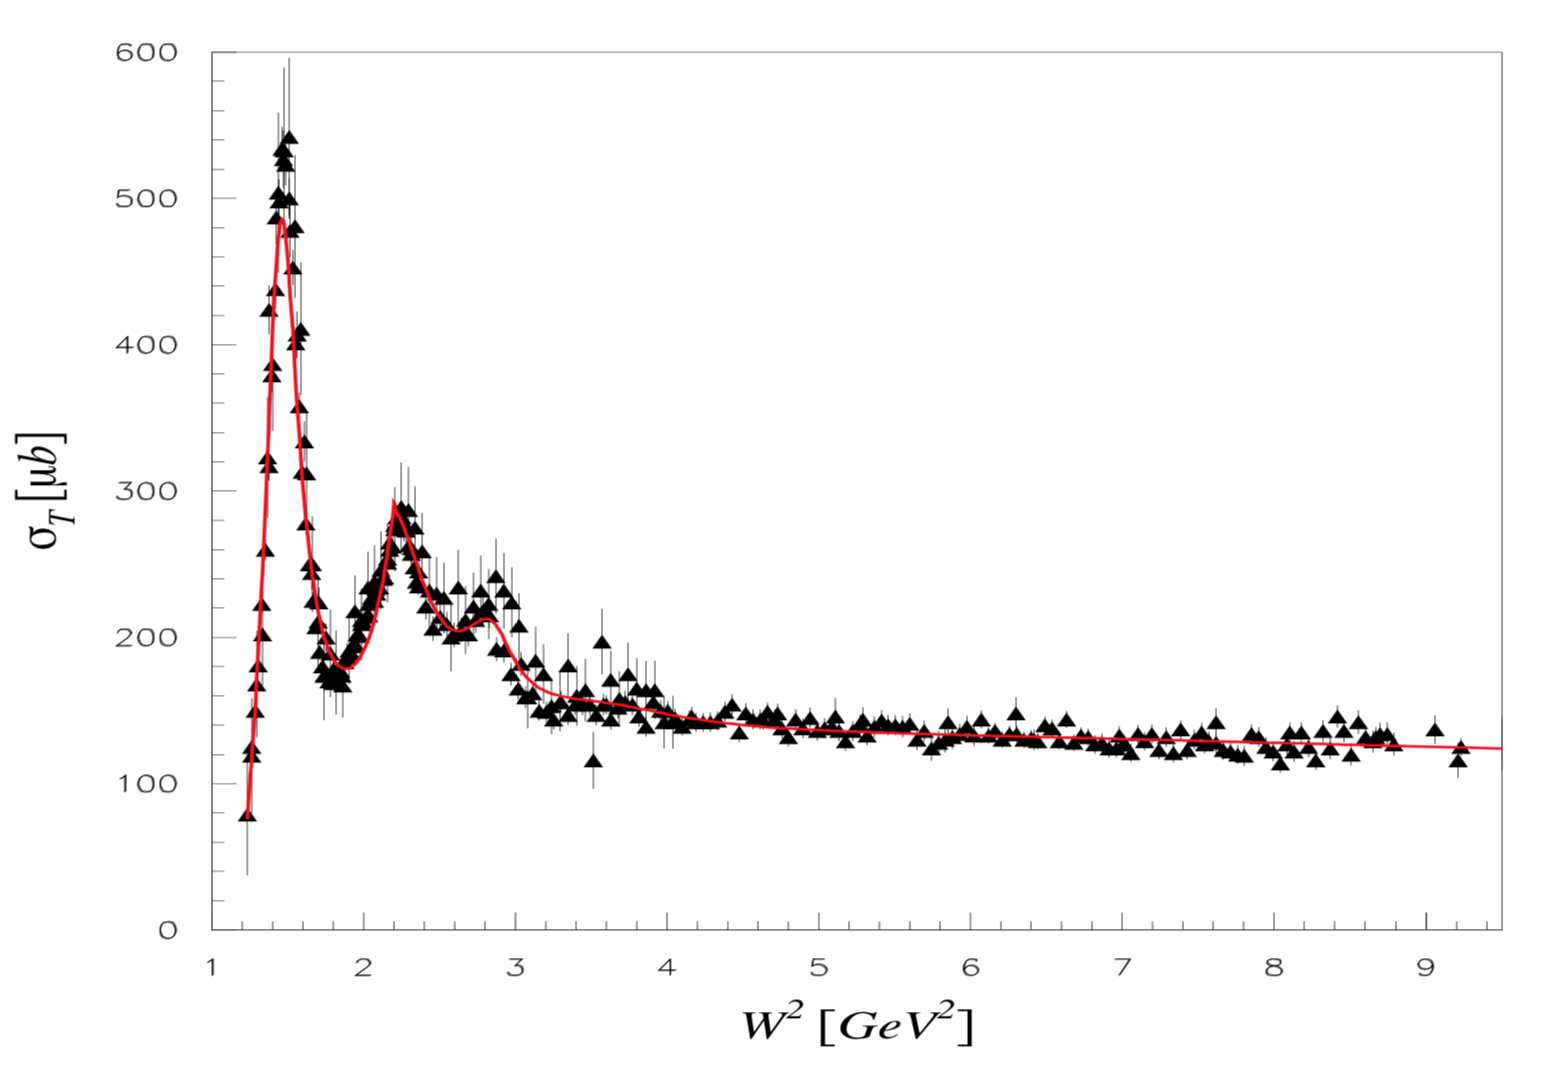
\includegraphics[width=0.9\linewidth]{figures/christy_bosted_fit.png}
	\caption[Total cross section vs. $W^2$ for existing data (black triangles) and the Christy-Bosted fit in red.]{Total cross section vs. $W^2$ for existing data (black triangles) and the Christy-Bosted fit in red \cite{christy_bosted}.}
	\label{fig:christy_bosted}
\end{figure}

The event generator uses the cross sections from the Christy-Bosted fit to create input files in LUND format that contain events from the inclusive DIS reaction $ep\rightarrow e'X$. Those LUND files are inputs to GEMC, which propagates the particles from the LUND file through the CLAS12 detectors to create raw Monte Carlo (MC) data. That data is then decoded and reconstructed using the same CLARA software as the RGA data.

\section{Fiducial Cuts}
Each detector has limits where it cannot efficiently detect particles. The edges of detectors are particularly vulnerable to inefficient and inconsistent particle detection. The goal of placing fiducial cuts on detectors is to remove from the data set events that are detected in areas of low or unknown efficiency. The Event Builder in CLARA does make cuts on detectors and kinematics in order to ensure the particle identification is efficient and the event occurs within the target area, with proper response in the forward detectors.

\begin{figure}[H]
	\centering
	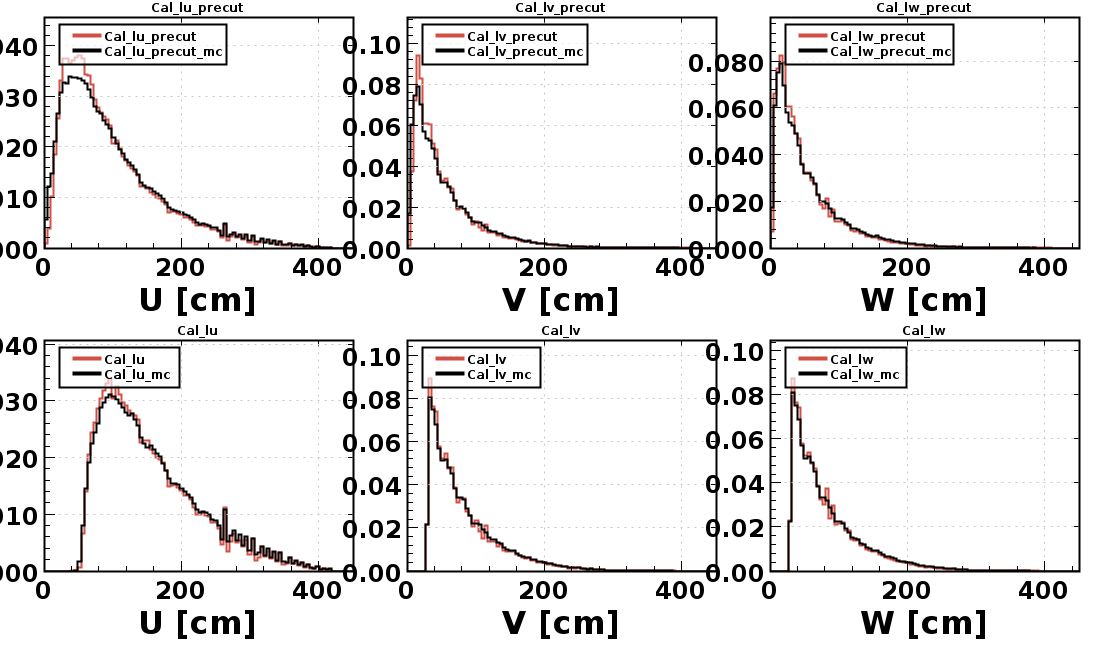
\includegraphics[width=0.9\linewidth]{figures/rga/1d_ecal.png}
	\caption{Count distributions of the U, V, and W dimensions of the pre-shower calorimeter (PCAL). The raw histograms are on the top and the bottom histograms contain the cuts: $U>30$ cm, $30<V<390$ cm, and $30<W<390$ cm. All plots are normalized to account for any mismatch in total statistics. Red lines are from RGA data and black lines are for the Monte-Carlo (MC) data.}
	\label{fig:rga_1decal}
\end{figure}

\begin{figure}[H]
	\centering
	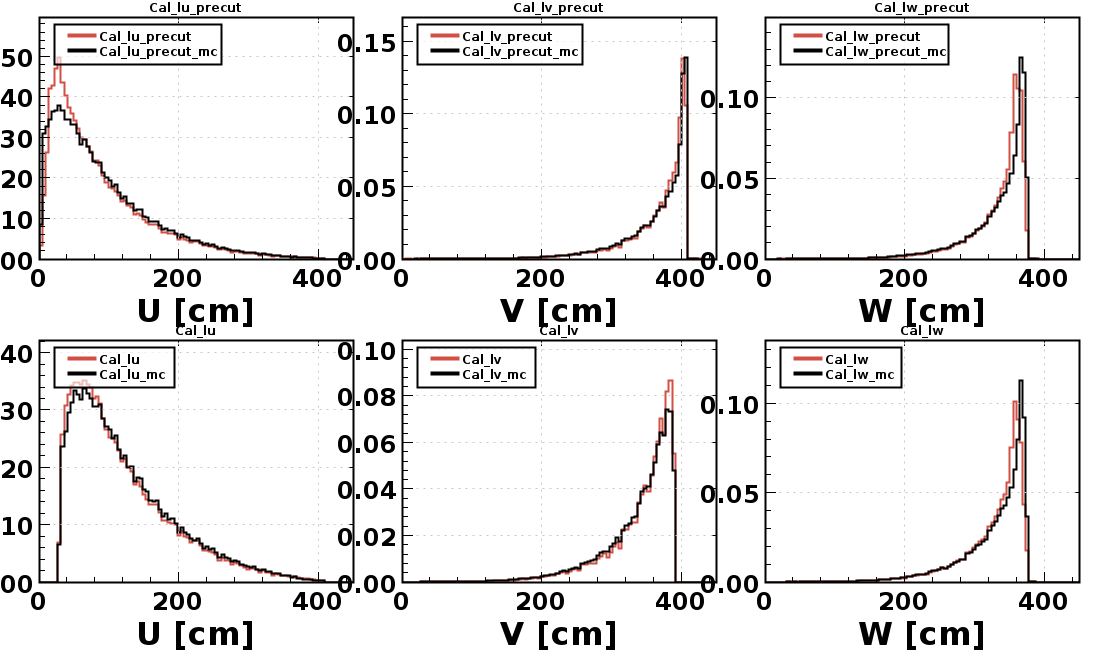
\includegraphics[width=0.9\linewidth]{figures/rga/1d_ecal_ECIN.png}
	\caption{Count distributions of the U, V, and W dimensions of the inner EC. The raw histograms are on the top and the bottom histograms contain the cuts on the PCAL: $U>30$ cm, $30<V<390$ cm, and $30<W<390$ cm. All plots are normalized to account for any mismatch in total statistics. Red lines are from RGA data and black lines are for the Monte-Carlo (MC) data.}
	\label{fig:rga_1decal_ecin}
\end{figure}

\begin{figure}[H]
	\centering
	\includegraphics[width=0.9\linewidth]{figures/rga/1d_ecal_ECout.png}
	\caption{Count distributions of the U, V, and W dimensions of the outer EC. The raw histograms are on the top and the bottom histograms contain the cuts on the PCAL: $U>30$ cm, $30<V<390$ cm, and $30<W<390$ cm. All plots are normalized to account for any mismatch in total statistics. Red lines are from RGA data and black lines are for the Monte-Carlo (MC) data.}
	\label{fig:rga_1decal_ecout}
\end{figure}

\begin{figure}[H]
	\centering
	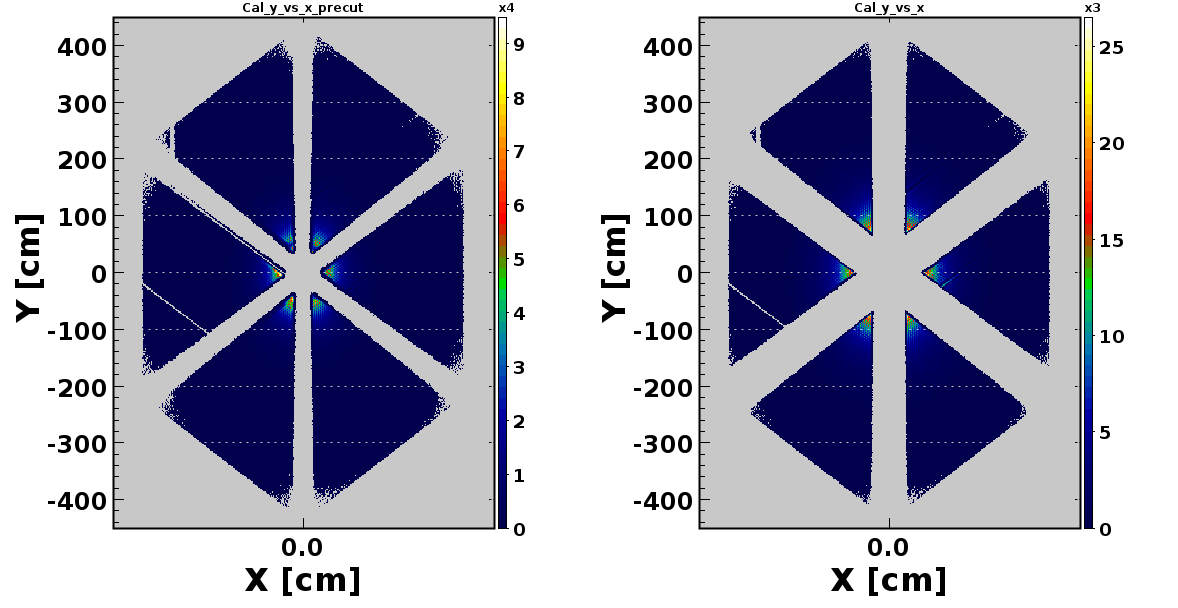
\includegraphics[width=0.9\linewidth]{figures/rga/2d_ecal.png}
	\caption{2D histograms of the uncut PCAL hits on the left and after the fiducial cuts are applied (right).}
	\label{fig:rga_2decal}
\end{figure}

\begin{figure}[H]
	\centering
	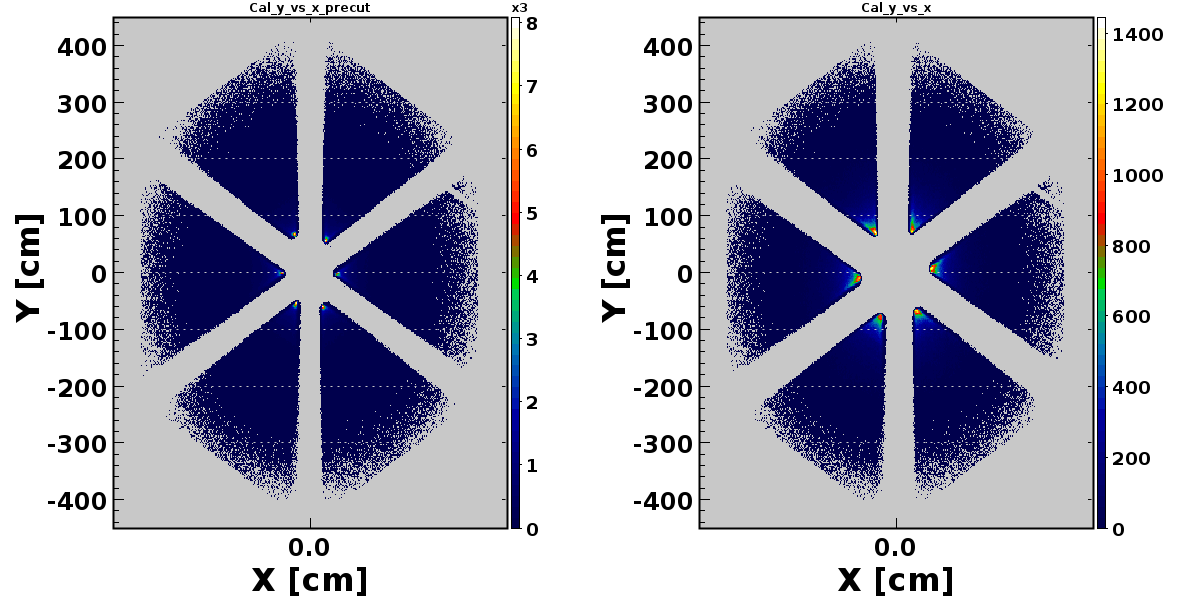
\includegraphics[width=0.9\linewidth]{figures/rga/2d_ecal_ECIN.png}
	\caption{2D histograms of the inner EC hits. On the left is before cuts on the PCAL, and on the right is after the fiducial cuts on the PCAL are applied.}
	\label{fig:rga_2decal_ecin}
\end{figure}

\begin{figure}[H]
	\centering
	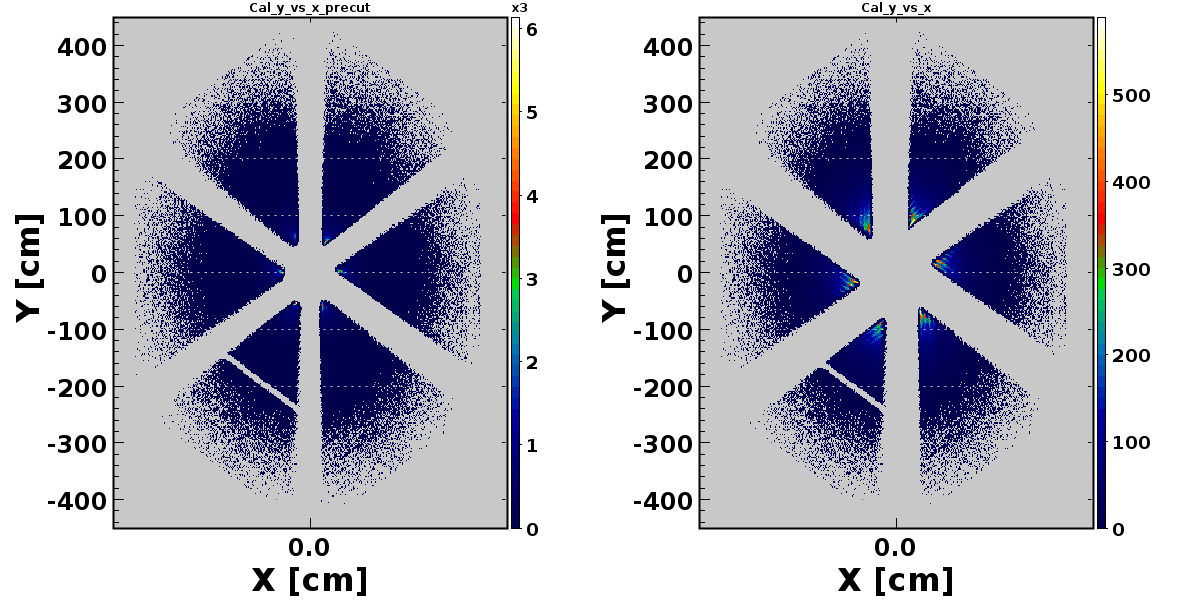
\includegraphics[width=0.9\linewidth]{figures/rga/2d_ecal_ECOUT.png}
	\caption{2D histograms of the outer EC hits. On the left is before cuts on the PCAL, and on the right is after the fiducial cuts on the PCAL are applied.}
	\label{fig:rga_2decal_ecout}
\end{figure}

The EC is the detector that we use for determining the scattered electron energy and all kinematics that are calculated from that energy. When electrons enter the EC they shower and stop. That EM shower is broad, so we have to remove events close to the edges since the total energy deposited is unreliable for $e^-$ identification in those cases. The Event Builder makes an $E_{\mathrm{PCAL}}>60$ MeV cut on the PCAL energy and a $-15<v_z<15$ cm vertex cut.

Remember that an EC detector is defined by U, V, and W edges of its triangular shape (see Section \ref{sec:EC}). We can cut on those edges for the PCAL only and the effects will propagate through to the EC$_{\mathrm{inner}}$ (ECin) and EC$_{\mathrm{outer}}$ (ECout) detectors. The established cuts for the PCAL are $U>30$ cm, $30<V<390$ cm, and $30<W<390$ cm. Fig. \ref{fig:rga_1decal} shows the count distributions of the U, V, and W sectors of the PCAL. Fig. \ref{fig:rga_1decal_ecin} shows the count distributions of the inner EC and Fig. \ref{fig:rga_1decal_ecout} shows the count distributions for the outer EC. For Figs. \ref{fig:rga_1decal}-\ref{fig:rga_1decal_ecout} the uncut histograms are on the top and the bottom histograms contain the PCAL cuts that were described. Fig. \ref{fig:rga_2decal} contains the two-dimensional histograms of the uncut PCAL hits on the left and the 2D histogram containing the fiducial cuts on the right. Fig. \ref{fig:rga_2decal_ecin} and Fig. \ref{fig:rga_2decal_ecout} show the 2D histograms for the inner EC and outer EC, respectively, with the uncut plots on the left and plots including PCAL cuts on the right. It is clear that there are less electrons that make it through the inner EC than the PCAL, and not as many make it through the outer EC than the inner EC.

\section{Kinematic and PID Cuts}
\label{sec:cuts}
Our goal is to extract the inclusive DIS cross section for the process $ep \longrightarrow e'X$, which means that certain constraints must be put on some of the kinematic variables. To isolate DIS events, we select $W>2$ GeV and $Q^2>1$ GeV$^2$. In order to isolate events that originate at the target, we require $-10 \; \mathrm{cm} < v_z < 10 \; \mathrm{cm}$, where $v_z$ is the z-vertex position of the track. Fig. \ref{fig:rga_vz} shows $v_z$ before (left) and after (right) cuts. It is clear that a $-15 \; \mathrm{cm} < v_z < 15 \; \mathrm{cm}$ cut was made during reconstruction.

\begin{figure}[h!]
	\centering
	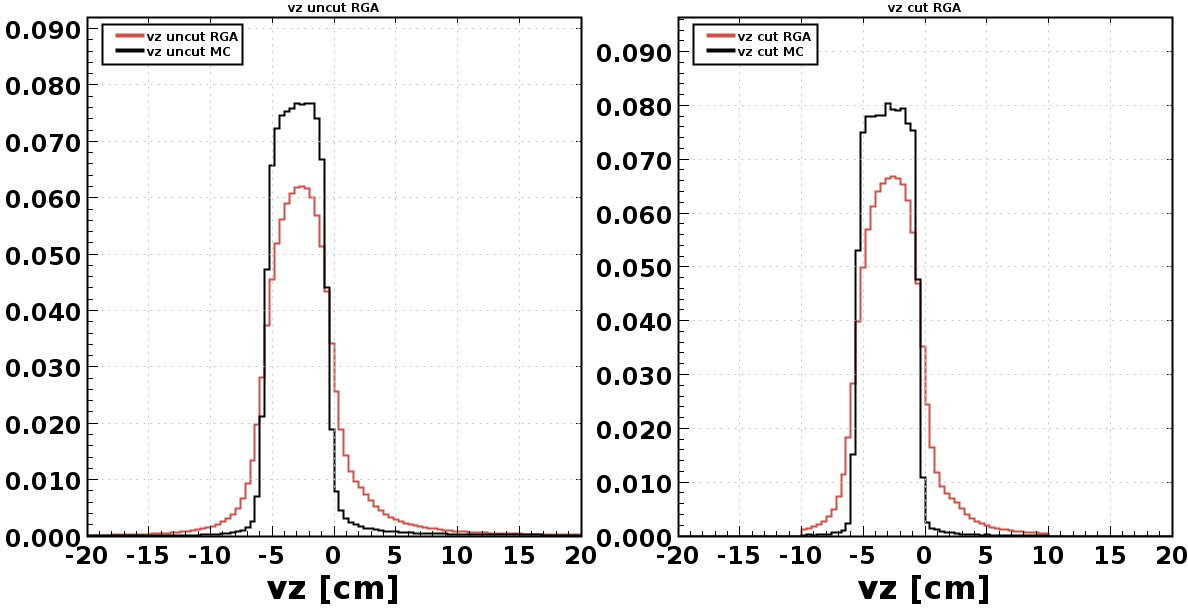
\includegraphics[width=0.9\linewidth]{figures/rga/vz.png}
	\caption{The electron vertex $v_z$ before (left) and after (right) all described cuts. Red lines are from RGA data and black lines are for the Monte-Carlo (MC) data.}
	\label{fig:rga_vz}
\end{figure}

\begin{figure}[h!]
	\centering
	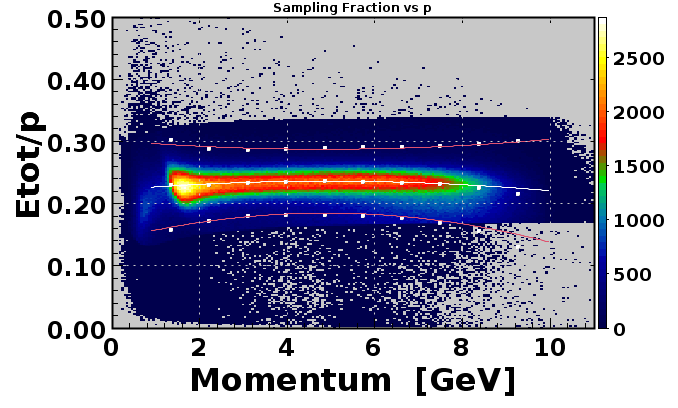
\includegraphics[width=0.9\linewidth]{figures/rga/fit_etot_p.png}
	\caption{Sampling fraction as a function of particle momentum. The dots represent the mean along the center and values $\pm2.5\sigma$ from that mean. The red lines are the fitted polynomials.}
	\label{fig:rga_etot_p}
\end{figure}

\begin{figure}[h!]
	\centering
	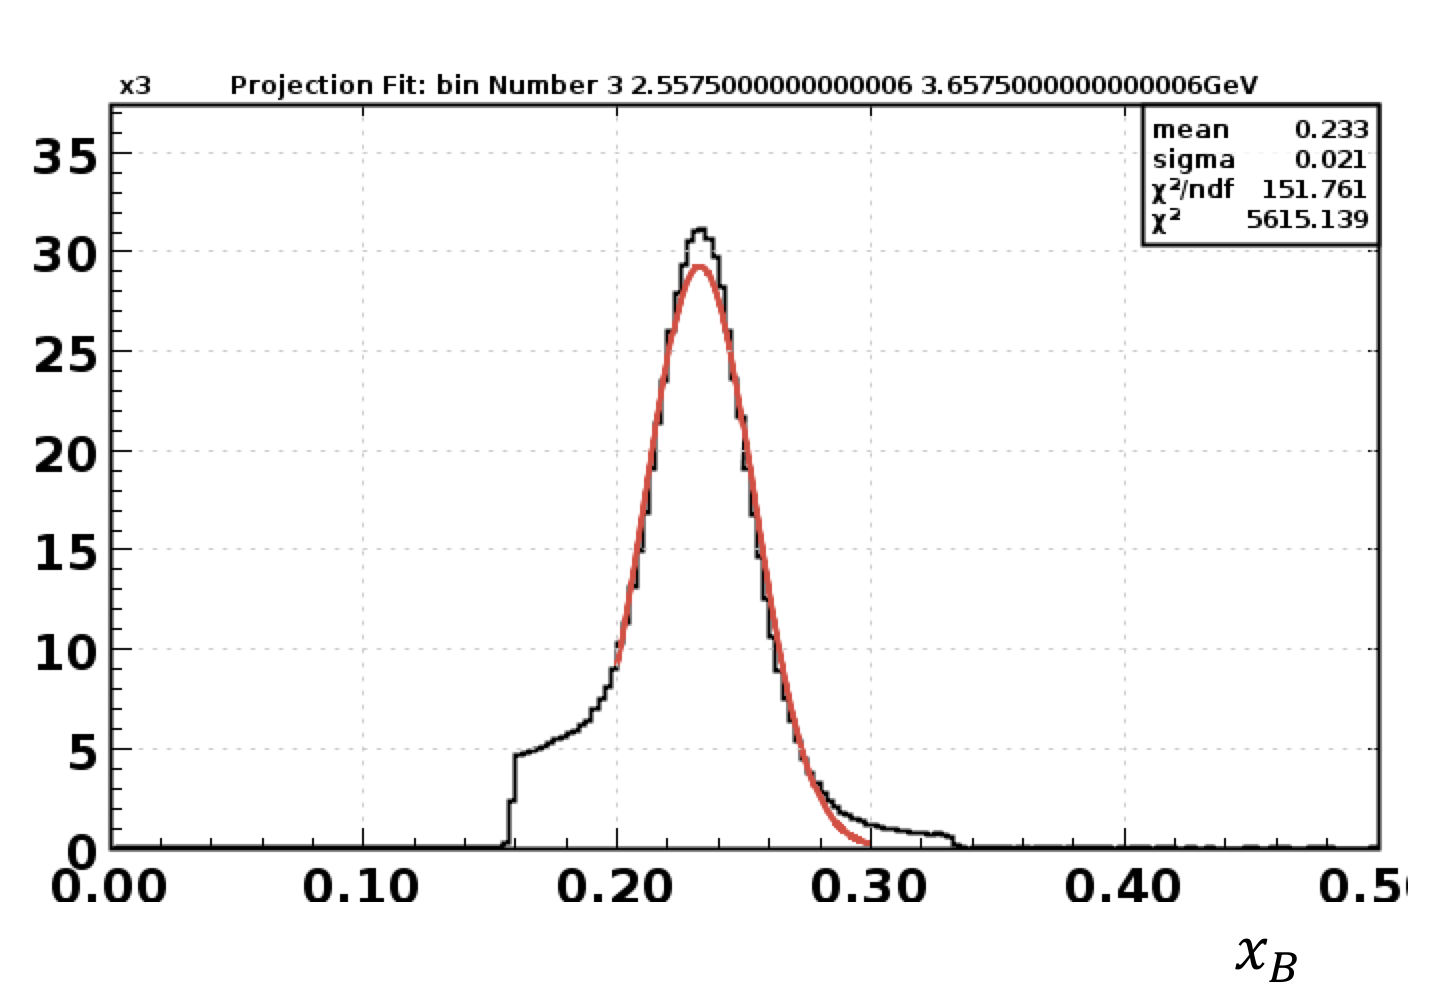
\includegraphics[width=0.9\linewidth]{figures/rga/Fit_slice_3.png}
	\caption{Slice of the sampling fraction for $2.58<p<3.66$ GeV fitted to a Gaussian. The sigma is used to find the $\pm2.5 \sigma$ fit seen in Fig. \ref{fig:rga_etot_p}.}
	\label{fig:sf_slice}
\end{figure}

The last significant cut occurs on the sampling faction. The sampling fraction is defined as $E_{tot}/p$, where $E_{tot}$ is the total energy deposited by the particle in both layers of the EC ($i.e.$ inner and outer EC) and $p$ is the particle's momentum as measured by the drift chambers. When the sampling fraction is plotted vs $p$, electrons will appear as a band around 0.25 $E_{tot}/p$. A selection of  momentum above 1 GeV was applied to eliminate any minimum ionizing particles like pions (see Fig. \ref{fig:rga_etot_p}). To select events near the band at 0.25, we take momentum slices of the data, find the mean and sigma of $E_{tot}/p$ for that slice and cut out events outside $\pm2.5\sigma$. Fig. \ref{fig:sf_slice} shows one of those slices with the Gaussian fit. This is done for values along $p$ and fit the points for means and $\pm2.5\sigma$ to polynomials. These two second-order polynomials are
\begin{equation}
\left( \frac{E_{\mathrm{tot}}}{p} \right)_{+2.5\sigma} = 0.0008p^2 - 0.0112p + 0.3137
\end{equation}
and
\begin{equation}
\left( \frac{E_{\mathrm{tot}}}{p} \right)_{-2.5\sigma}  = -0.0017p^2 + 0.0228p + 0.1397
\end{equation}
for $+2.5\sigma$ and $-2.5\sigma$, respectively.

Because of the Forward Detector's coverage in $\theta$, we apply an additional $5^{\circ} < \theta < 40^{\circ}$ cut on that variable. Fig. \ref{fig:rga_kinematics_uncut} shows the uncut kinematic variables and Fig. \ref{fig:rga_kinematics_cut} was created with the kinematic cuts described. Fig. \ref{fig:rga_energies_uncut} and Fig. \ref{fig:rga_energies} shows uncut and cut (respectively) distributions for $E'$, $E_{\mathrm{ECin}}$, $E_{\mathrm{ECout}}$, $E_{\mathrm{PCAL}}$, $E_{\mathrm{ECtot}}$, and the number of photoelectrons in the HTCC ($nphe$). The total energy deposited in the EC ($i.e.$ $E_{\mathrm{ECtot}}$) is the addition of $E_{\mathrm{ECin}}$ and $E_{\mathrm{ECout}}$. The next group of plots Figs. \ref{fig:rga_2Dkin1_uncut}-\ref{fig:rga_sampFrac} shows two-dimensional histograms of various kinematic variables all uncut and after applying all cuts. In Fig. \ref{fig:rga_sampFrac} one can clearly see the successful application of the $5\sigma$ cut described in the previous paragraph. The summary of applied cuts is as follows:
\newpage
\noindent
\textbf{DIS Kinematics}
\begin{itemize}
	\item $W>2$ GeV
	\item $Q^2>1$ GeV$^2$
\end{itemize}
\textbf{Fiducial}
\begin{itemize}
	\item PCAL cuts: $U>30$ cm, $30<V<390$ cm, and $30<W<390$ cm
	\item $-10<v_z<10$ cm
	\item $5^{\circ} < \theta < 40^{\circ}$
\end{itemize}
\textbf{Particle ID ($e^-$ selection)}
\begin{itemize}
	\item $5\sigma$ cut on sampling fraction
	\item HTCC cut: $nphe > 5$
	\item EC energy cuts: $E_{\mathrm{PCAL}} > 0.06$ GeV, $E_{\mathrm{EC_{in}}} > 0.025$ GeV, $E_{\mathrm{EC_{out}}} > 0.05$ GeV
\end{itemize}

There are clearly cuts applied during reconstruction ($i.e.$ before the data analysis described here). These cuts occur in the Event Builder whose job it is to build tracks and identify particles. Some of the cuts that were described in this section to identify DIS electrons are used to identify all electrons. For example, in order to ensure a clear signal in the HTCC, the EB uses a cut below 2 photoelectrons (or 2 nphe) to assist in $e^-$ PID. After the described cuts, the data agreed well with the MC data, with a few exceptions. The energy distributions for $E_{\mathrm{PCAL}}$ and $E_{\mathrm{ECin}}$ in Fig. \ref{fig:rga_energies} shows differences between RGA data and MC data, the cause of which remains unknown. In that same figure, there is a disagreement in the number of photoelectrons ($nphe$) in the HTCC between RGA and MC data. The reason for this also remains elusive.

\begin{figure}[h!]
	\centering
	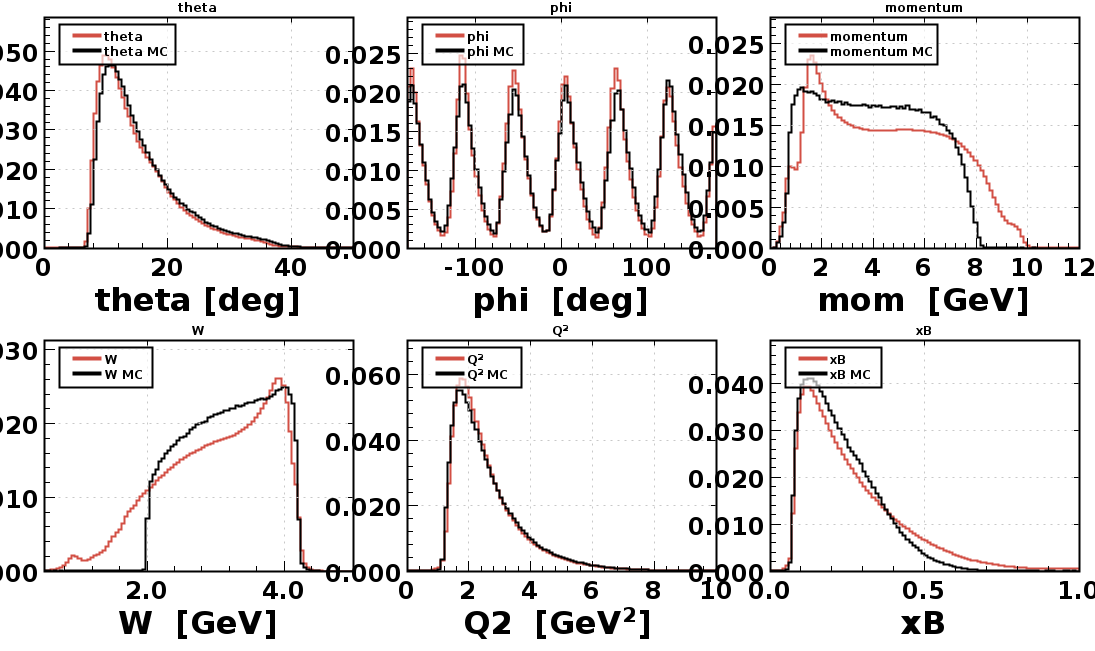
\includegraphics[width=0.9\linewidth]{figures/rga/uncut/kinematics.png}
	\caption{Kinematic variables before cuts. Red lines are from RGA data and black lines are for the Monte-Carlo (MC) data.}
	\label{fig:rga_kinematics_uncut}
\end{figure}

\begin{figure}[h!]
	\centering
	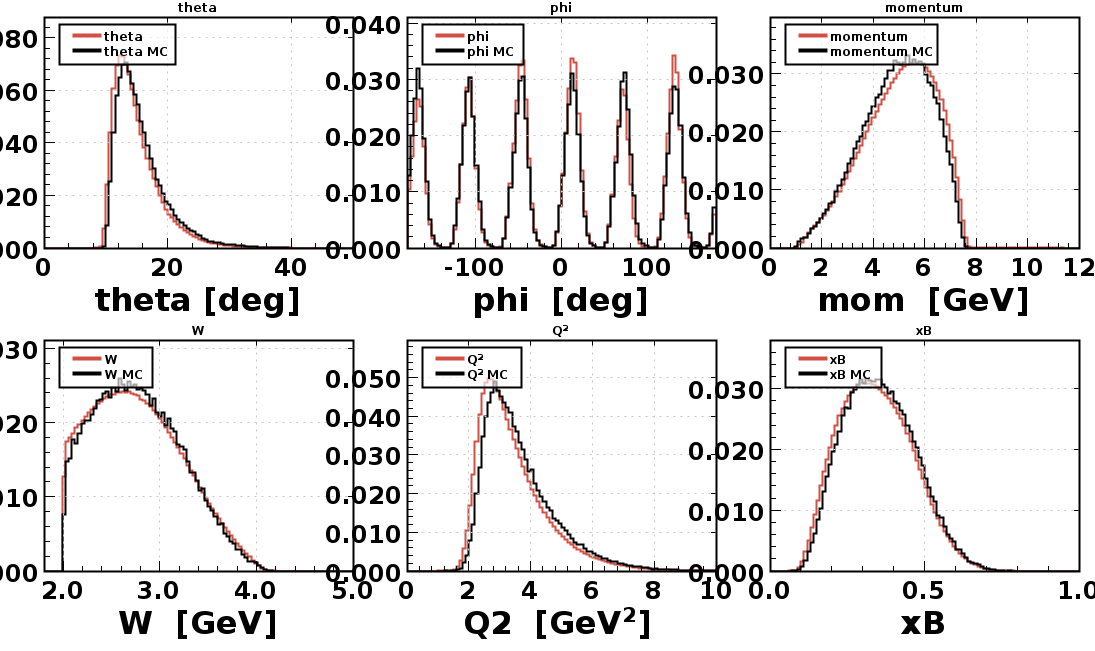
\includegraphics[width=0.9\linewidth]{figures/rga/kinematics.png}
	\caption{Kinematic variables after all described cuts. Red lines are from RGA data and black lines are for the Monte-Carlo (MC) data.}
	\label{fig:rga_kinematics_cut}
\end{figure}

\newpage
\begin{figure}[h!]
	\centering
	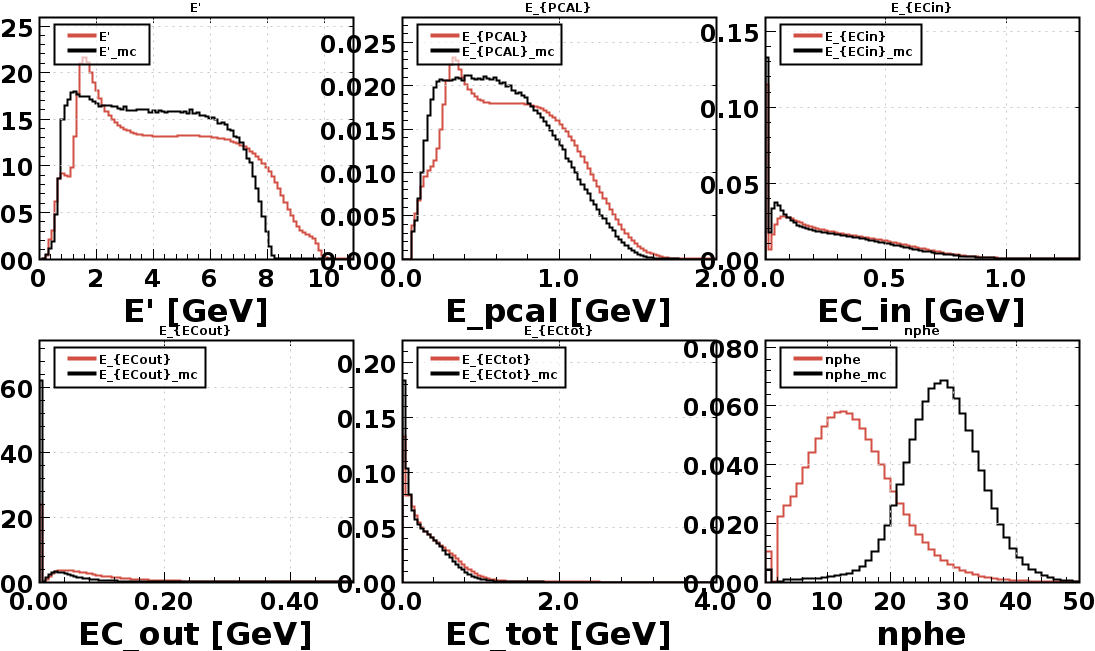
\includegraphics[width=0.9\linewidth]{figures/rga/uncut/energies.png}
	\caption{$E^{\prime}$, EC energies, and nphe before cuts. Red lines are from RGA data and black lines are for the Monte-Carlo (MC) data.}
	\label{fig:rga_energies_uncut}
\end{figure}

\begin{figure}[h!]
	\centering
	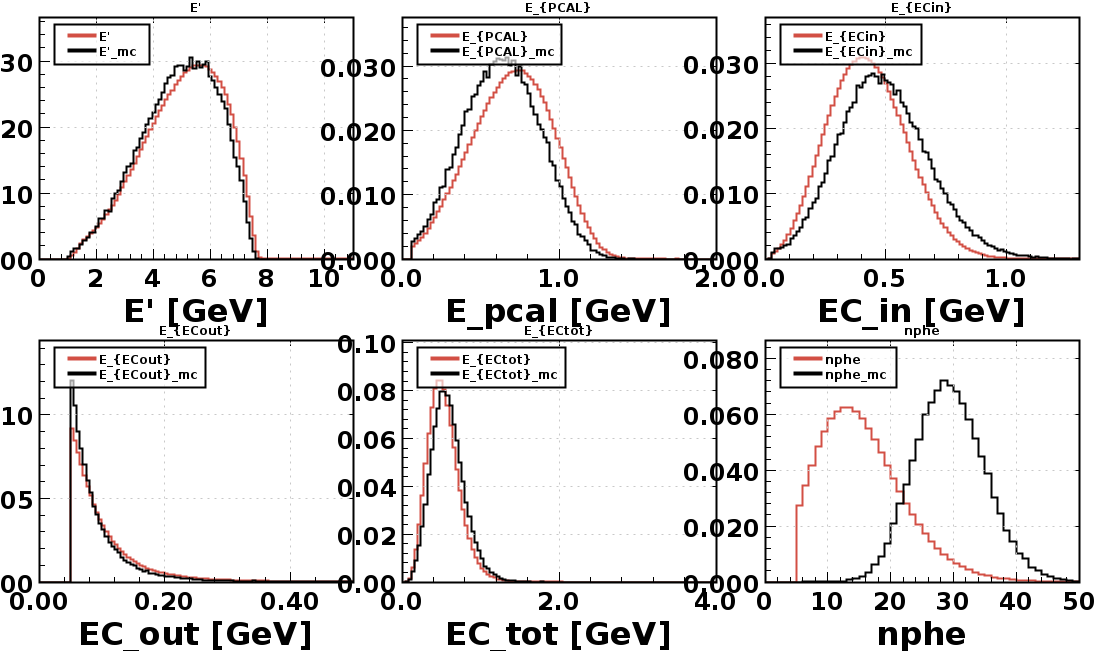
\includegraphics[width=0.9\linewidth]{figures/rga/energies.png}
	\caption{$E^{\prime}$, EC energies, and nphe after all described cuts. Red lines are from RGA data and black lines are for the Monte-Carlo (MC) data.}
	\label{fig:rga_energies}
\end{figure}

\newpage
\begin{figure}[h!]
	\centering
	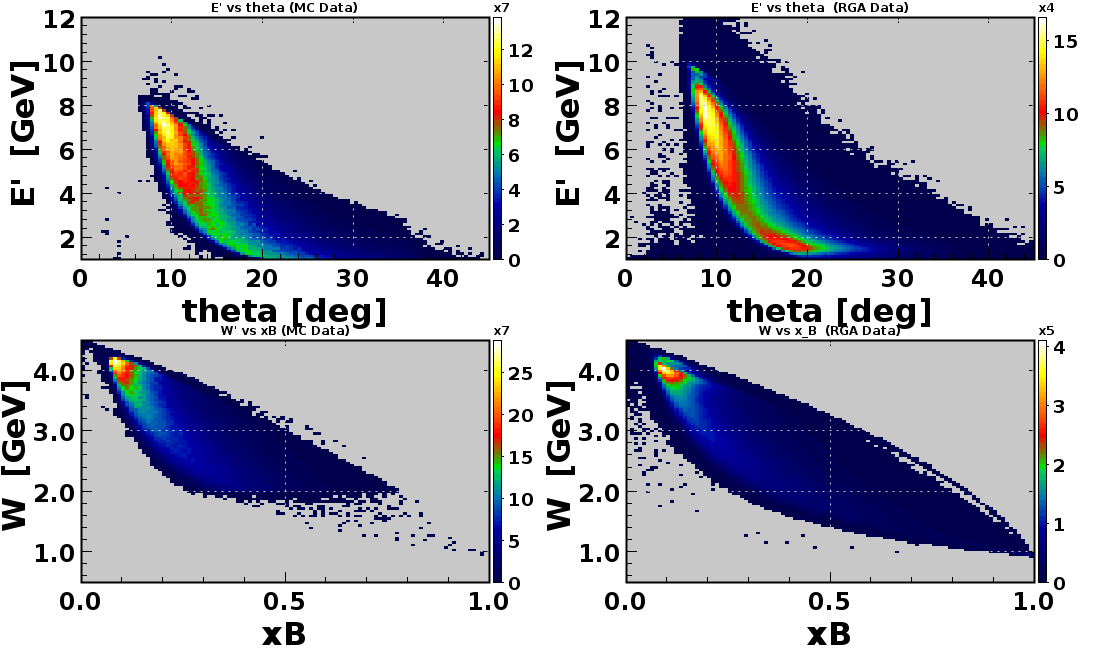
\includegraphics[width=0.9\linewidth]{figures/rga/uncut/2Dkin1.png}
	\caption{$E'$ vs. $\theta$ and $W$ vs. $x_B$ before cuts. The Monte Carlo data is on the left and the RGA data is on the right.}
	\label{fig:rga_2Dkin1_uncut}
\end{figure}

\begin{figure}[h!]
	\centering
	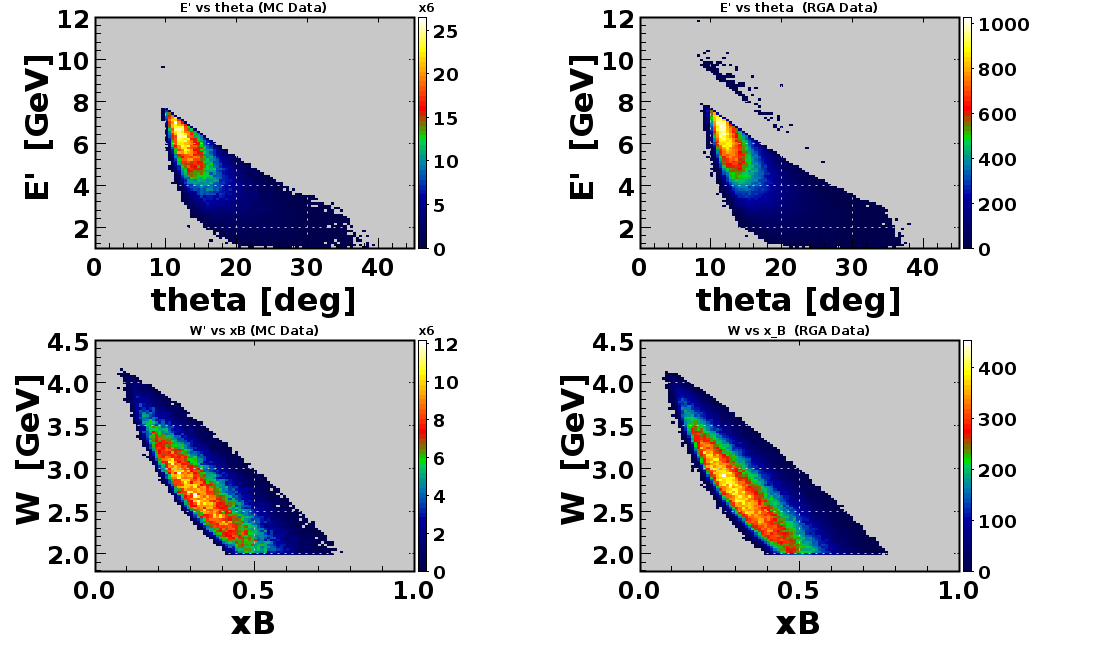
\includegraphics[width=0.9\linewidth]{figures/rga/2Dkin1.png}
	\caption{$E'$ vs. $\theta$ and $W$ vs. $x_B$ after all described cuts. The Monte Carlo data is on the left and the RGA data is on the right.}
	\label{fig:rga_2Dkin1}
\end{figure}

\newpage
\begin{figure}[h!]
	\centering
	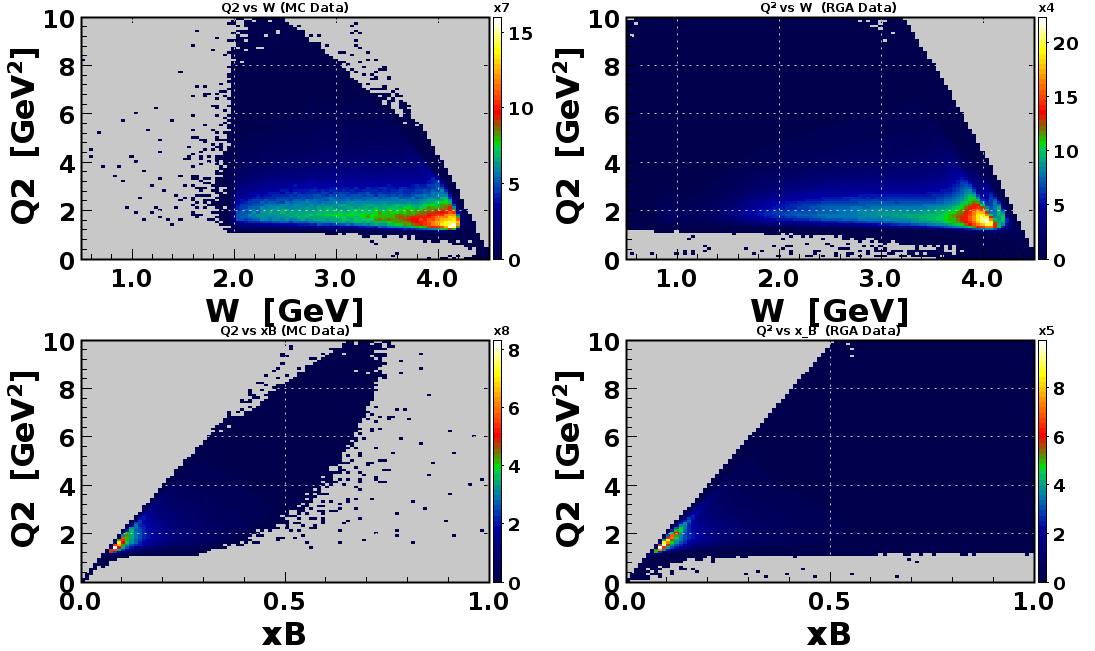
\includegraphics[width=0.9\linewidth]{figures/rga/uncut/2Dkin2.png}
	\caption{$Q^2$ vs. $W$ and $Q^2$ vs $x_B$ before cuts. The Monte Carlo data is on the left and the RGA data is on the right.}
	\label{fig:rga_2Dkin2_uncut}
\end{figure}

\begin{figure}[h!]
	\centering
	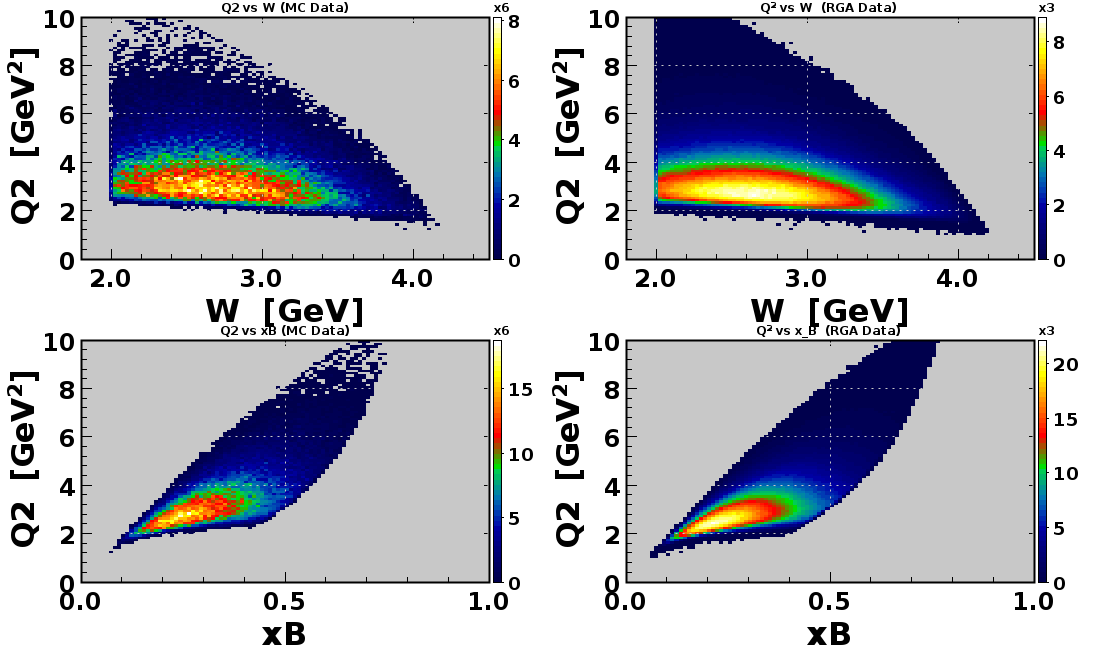
\includegraphics[width=0.9\linewidth]{figures/rga/2Dkin2.png}
	\caption{$Q^2$ vs. $W$ and $Q^2$ vs $x_B$ after all described cuts. The Monte Carlo data is on the left and the RGA data is on the right.}
	\label{fig:rga_2Dkin2}
\end{figure}

\newpage
\begin{figure}[h!]
	\centering
	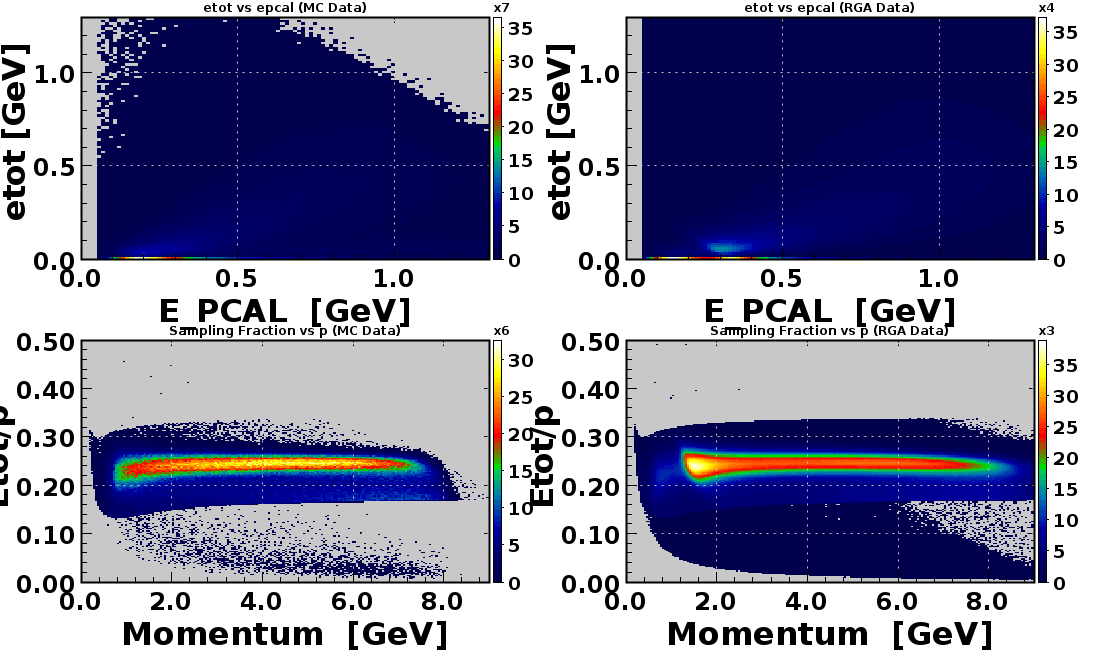
\includegraphics[width=0.9\linewidth]{figures/rga/uncut/sampFrac.png}
	\caption{$E_{EC_{tot}}$ vs $E_{PCAL}$ and Sampling fraction vs. $p$ before cuts. The Monte Carlo data is on the left and the RGA data is on the right.}
	\label{fig:rga_sampFrac_uncut}
\end{figure}

\begin{figure}[h!]
	\centering
	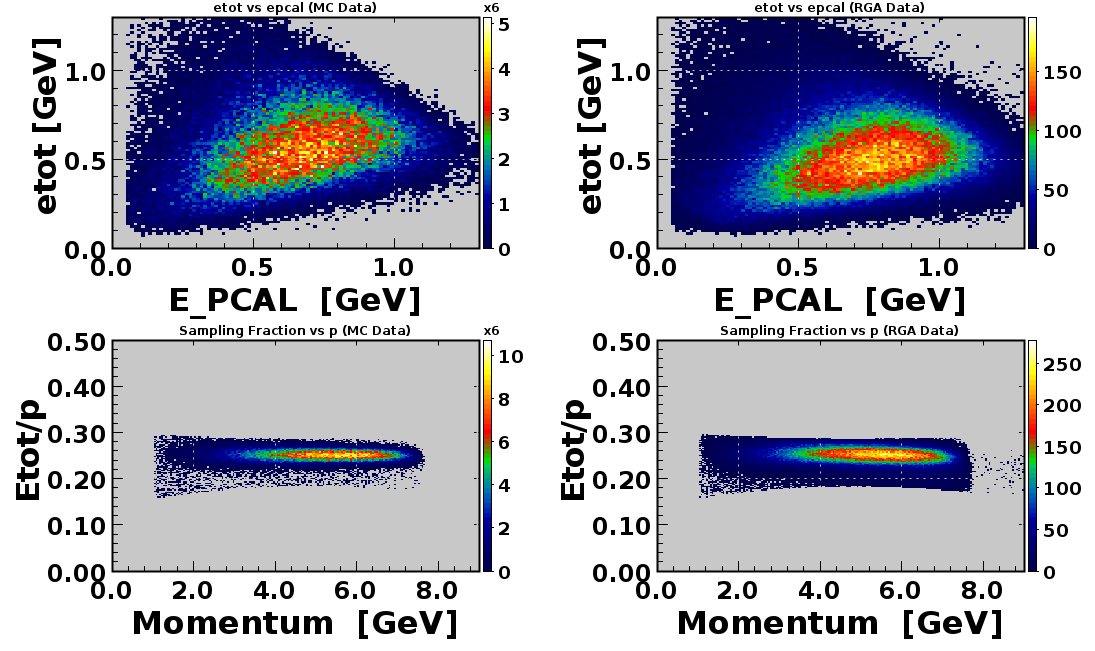
\includegraphics[width=0.9\linewidth]{figures/rga/sampFrac.png}
	\caption{$E_{EC_{tot}}$ vs $E_{PCAL}$ and Sampling fraction vs. $p$ after all described cuts. The Monte Carlo data is on the left and the RGA data is on the right.}
	\label{fig:rga_sampFrac}
\end{figure}

\cleardoublepage
\section{Binning and Acceptance}
The data, after kinematic and fiducial cuts, needs to be separated into kinematic bins in order to first obtain the acceptance of the bin and then to extract the cross section for each bin. The acceptance for the bin is the probability that an event in that bin will be successfully reconstructed in CLAS12. The acceptance can be determined using simulated (Monte Carlo) data:
\begin{equation}
A(x,y) = \frac{N_{\mathrm{rec}}(x,y)}{N_{\mathrm{gen}}(x,y)},
\end{equation}
where $A(x,y)$ is the acceptance of the bin, $N_{\mathrm{gen}}(x,y)$ is the number of generated events in that bin, and $N_{\mathrm{rec}}(x,y)$ is the number of reconstructed events in that bin. The binning occurs in $x$ ($i.e.$ the Bjorken-$x$ scaling variable) and $y$, which is defined as $y = \nu/E$. This particular binning was chosen because of the form of the cross section used by Christy-Bosted \cite{christy_bosted}, who parameterized existing data to the inclusive cross section, namely:
\begin{equation}
\label{eq:dis_xsec}
\frac{d^2\sigma}{dxdy} = \frac{4\pi\alpha_{\mathrm{em}}S}{Q^4} \left[ xy^2 F_1(x,Q^2) + \left( 1-y-xy\frac{M^2}{S} \right) F_2(x,Q^2) \right],
\end{equation}
where $S = 2ME$.

\begin{figure}[h!]
	\centering
	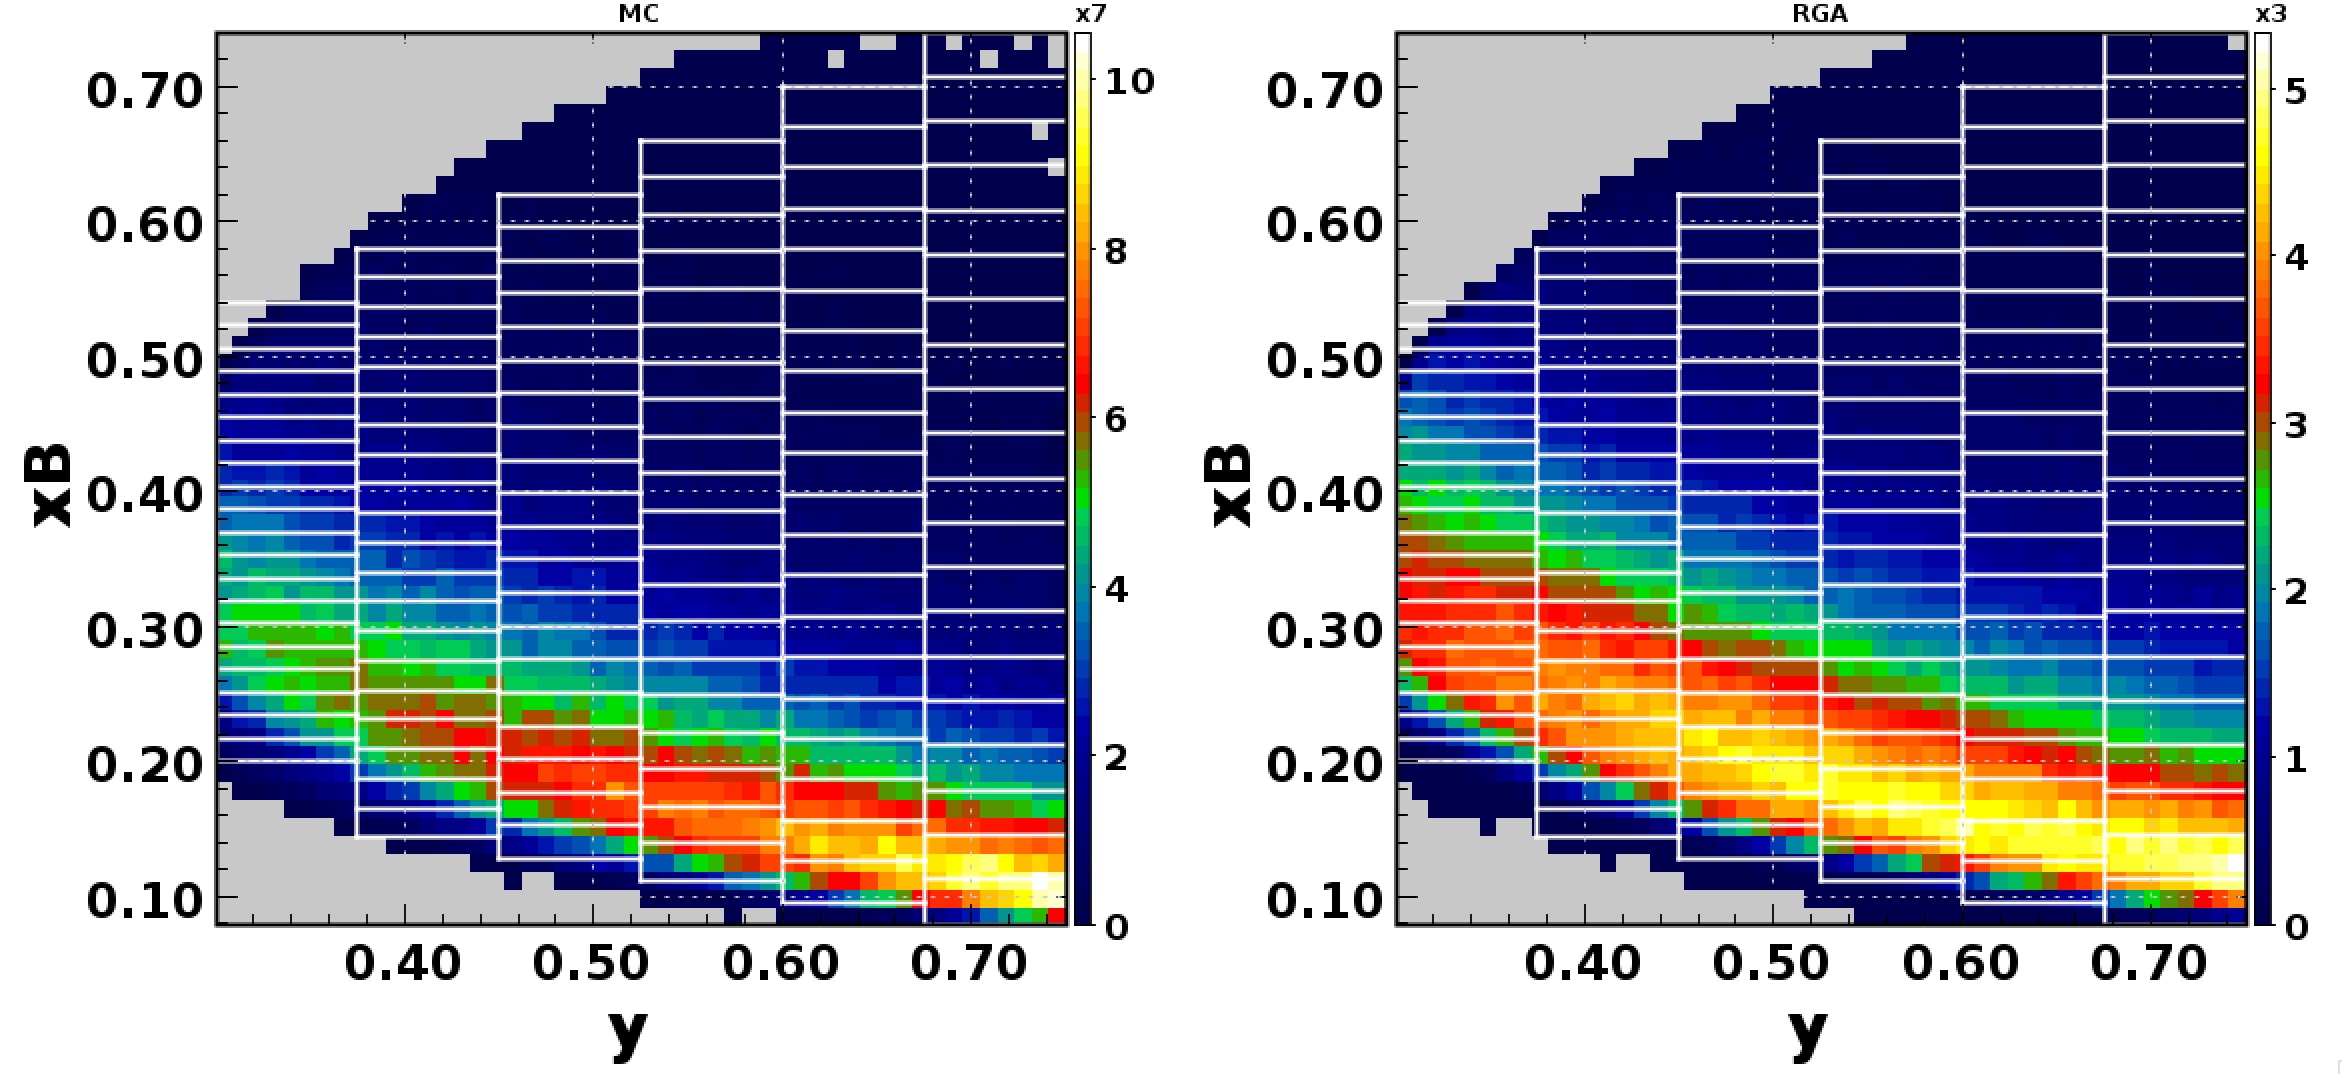
\includegraphics[width=0.9\linewidth]{figures/rga/xB_vs_y_bins.png}
	\caption{Binning in the $x,y$ space for MC data (left) and RGA Run 5036 data (right). These plots contain all events that pass the inclusive DIS cuts imposed as described in Section \ref{sec:cuts}.}
	\label{fig:xb_vs_y_bins}
\end{figure}

The binning in $x$ and $y$ was done in an attempt to ensure there were reasonable statistics in each bin. Equal bins were chosen in $y$ because the distribution was relatively flat in the range $0.3 < y < 0.74$. In $x$, however, the distribution in each $y$ bin required binning within different ranges of $x$. Table \ref{table:xB_bins} outlines the bin size and range for $x$. Fig. \ref{fig:xb_vs_y_bins} shows the binning in the $x,y$ space. 

\begin{table}[h!]
	\centering
	\begin{tabular}{ |c|c|c|c|c| } 
		\hline
		Bin & $y$ Range & $x_{\mathrm{min}}$ & $x_{\mathrm{max}}$ & $\Delta x$ \\
		\hline
		1 & 0.3-0.375 & 0.2 & 0.54 & 0.017 \\
		2 & 0.375-0.45 & 0.144 & 0.58 & 0.0218 \\
		3 & 0.45-0.525 & 0.128 & 0.62 & 0.0246 \\
		4 & 0.525-0.6 & 0.112 & 0.66 & 0.0274 \\
		5 & 0.6-0.675 & 0.096 & 0.7 & 0.0302 \\
		6 & 0.675-0.74 & 0.08 & 0.74 & 0.033 \\
		\hline
	\end{tabular}
	\caption{Summary of binning in $x$ and $y$.}
	\label{table:xB_bins}
\end{table}

Figs. \ref{fig:rga_acc0}-\ref{fig:rga_acc2} show the acceptance for each bin. For each bin in $y$, the value of which is located in the caption of each plot, the acceptance is then plotted for each bin in $x$. The error on the acceptance is calculated using
\begin{equation}
\delta A(x,y) = \frac{A(x,y)}{\sqrt{N_{\mathrm{rec}}}}
\end{equation}
Ideally the acceptance for all bins would be unity, but in practice the CLAS12 detector cannot reconstruct all events because of geometric and detector limitations. It is clear that the acceptance in some bins is low. In fact, the first bin in $x$ for each $y$ bin was so low that those data points were omitted. In Fig. \ref{fig:rga_acc0} we see that the acceptance is low at $x \rightarrow 0$ and in Fig. \ref{fig:rga_acc2} acceptance drops as $x \rightarrow 1$.

\begin{figure}[h!]
	\centering
	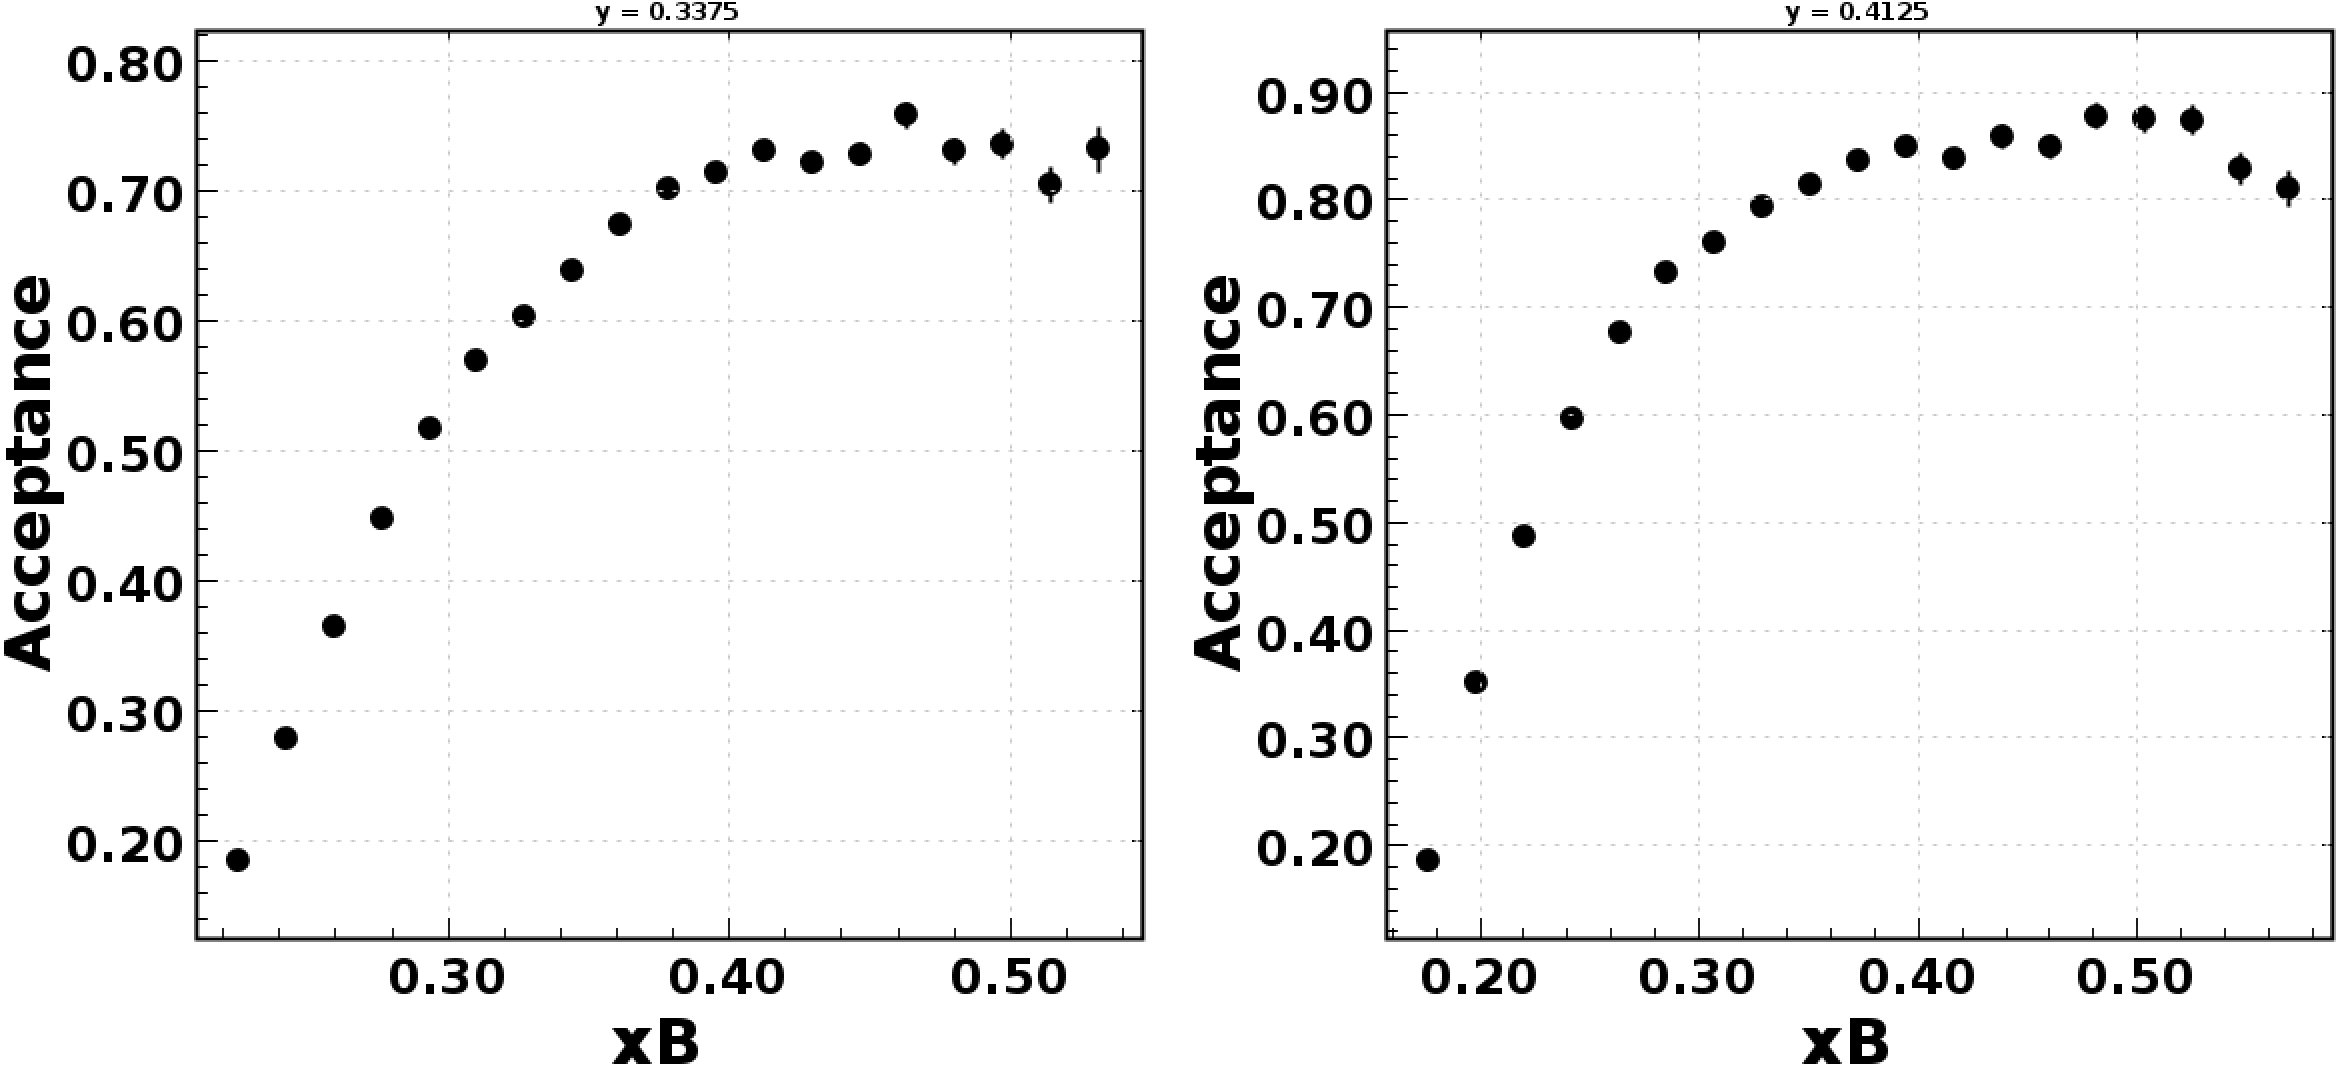
\includegraphics[width=0.9\linewidth]{figures/rga/acceptance0.png}
	\caption{Acceptance for $y=$0.3375 (left) and $y=$0.4175 (right) $vs$ $x$.}
	\label{fig:rga_acc0}
\end{figure}
\begin{figure}[h!]
	\centering
	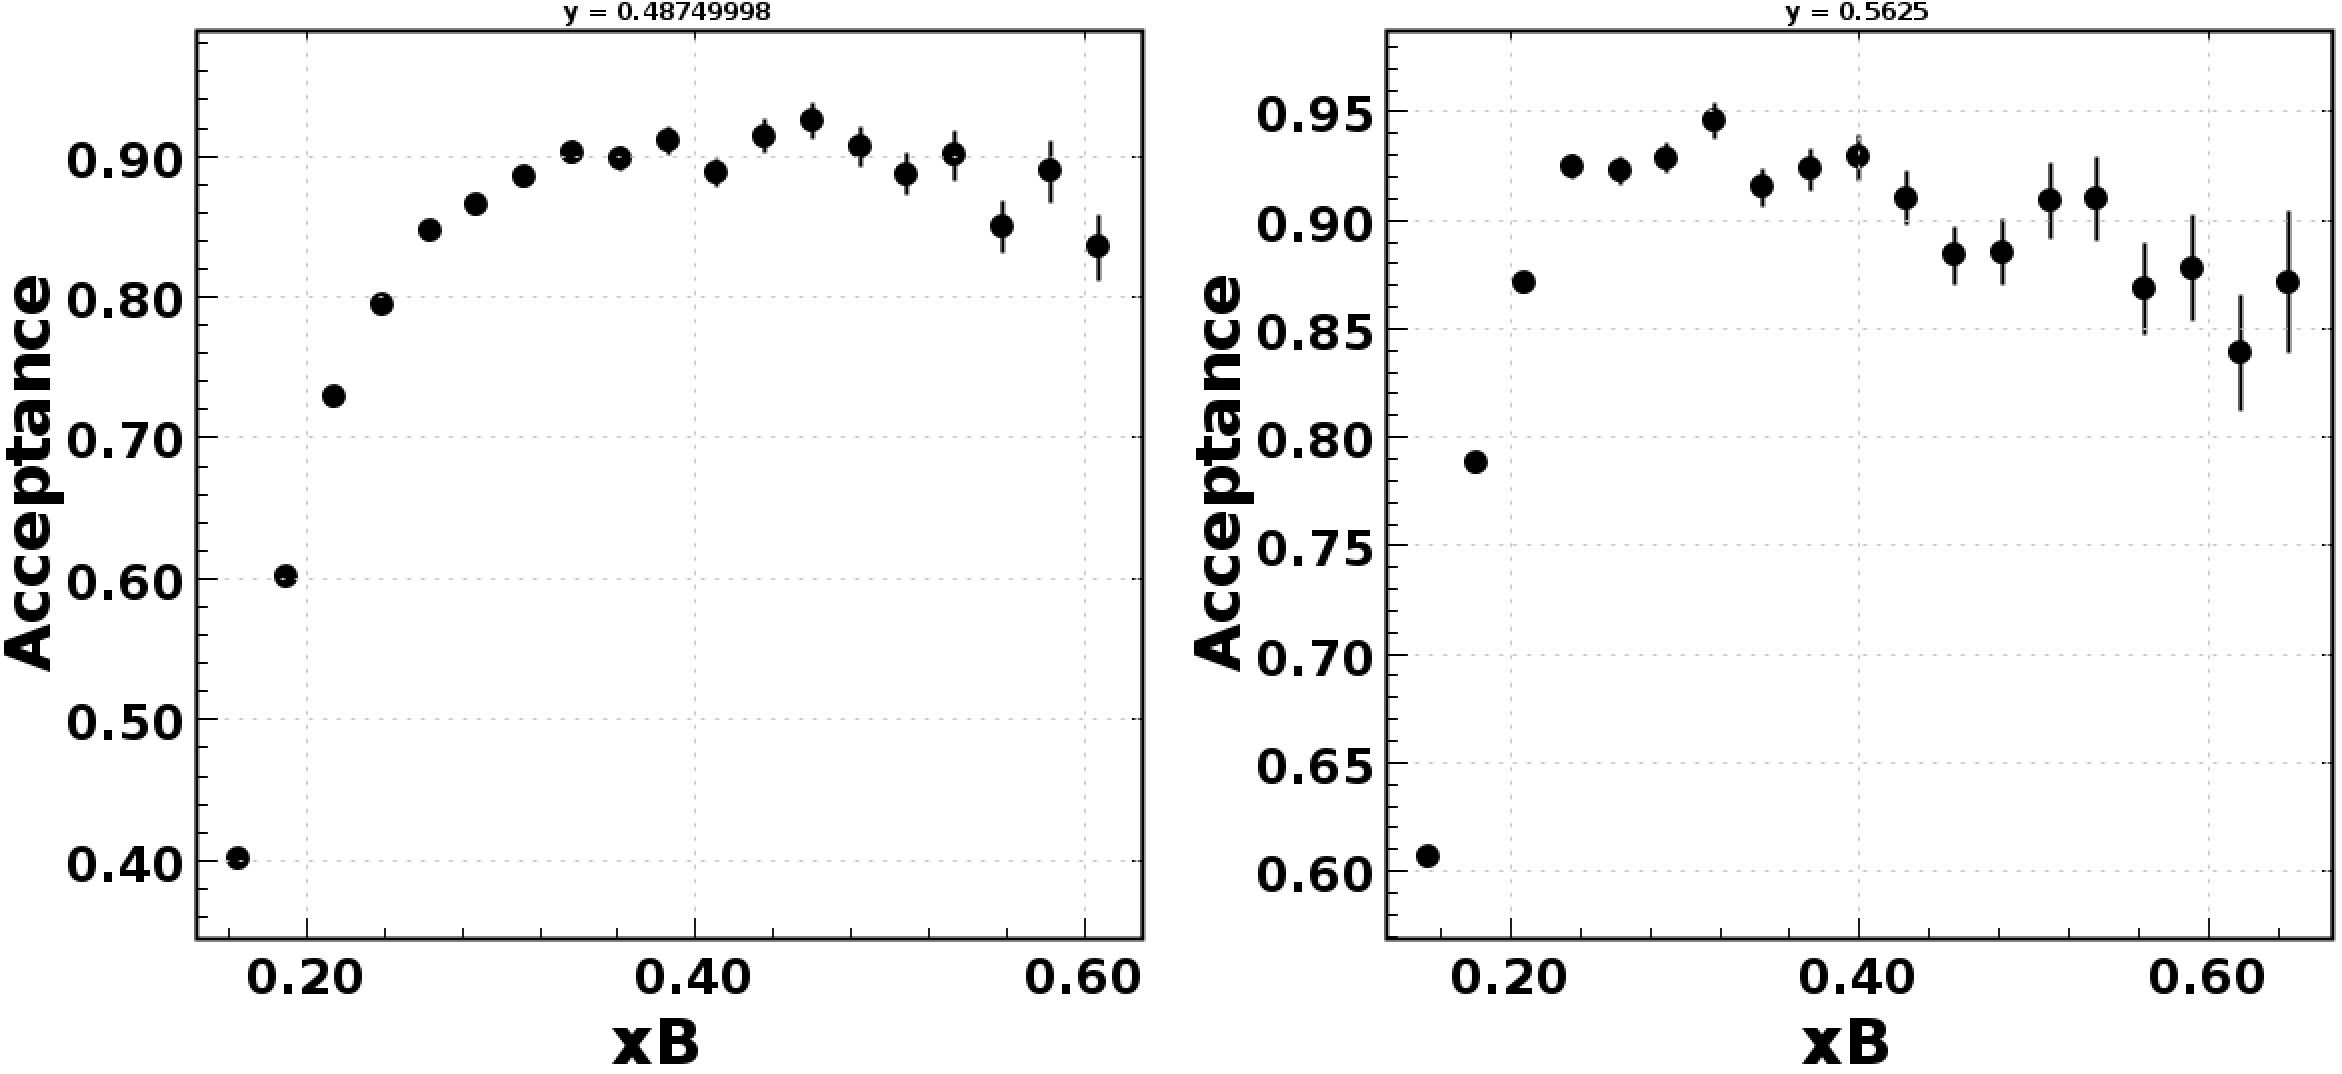
\includegraphics[width=0.9\linewidth]{figures/rga/acceptance1.png}
	\caption{Acceptance for $y=$0.4875 (left) and $y=$0.5625 (right) $vs$ $x$.}
	\label{fig:rga_acc1}
\end{figure}
\begin{figure}[h!]
	\centering
	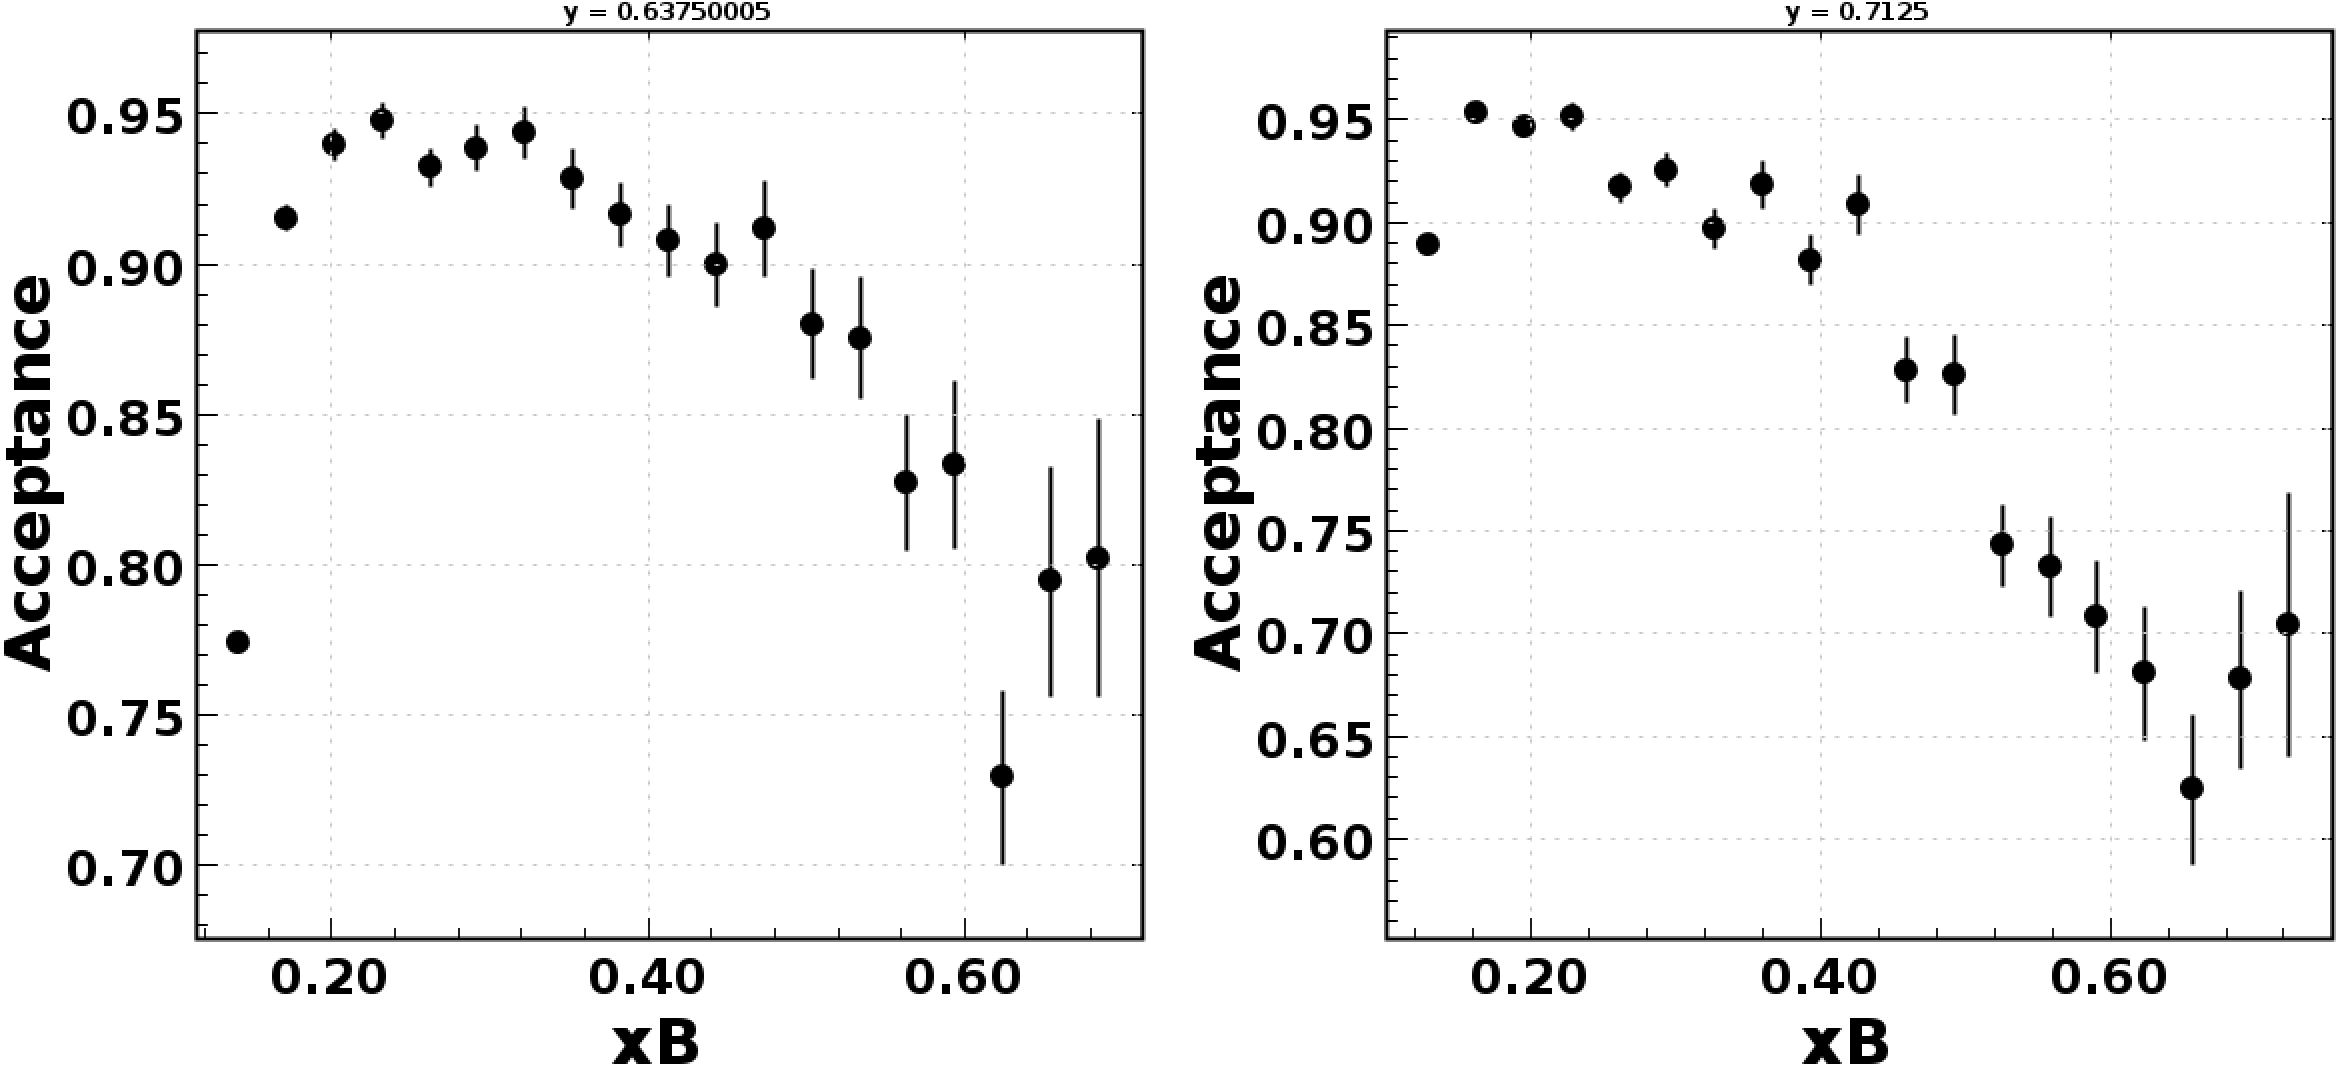
\includegraphics[width=0.9\linewidth]{figures/rga/acceptance2.png}
	\caption{Acceptance for $y=$0.6375 (left) and $y=$0.7125 (right) $vs$ $x$.}
	\label{fig:rga_acc2}
\end{figure}

\section{Faraday Cup and Integrated Luminosity}
As will become more evident in the next section, cross section extraction from data depends on the number of beam electrons accumulated during a particular run. Since the cross section is the probability that a reaction occurs for a given process, it also depends on the number of target nuclei. The \textit{luminosity} ($\mathscr{L}$) is a quantity that incorporates both accumulated charge and the number of target nuclei by expressing the number of beam particles per time multiplied by the number of target nuclei per unit area. By integrating that luminosity over time, we can recover the total number of beam electrons multiplied by the number of target nuclei per unit area
\begin{equation}
\mathscr{L_{\mathrm{int}}} = \int \mathscr{L} \; dt = \frac{N_{B} \times N_{\mathrm{target}}}{A},
\end{equation}
where $N_{B}$ is the total number of incident electrons, $N_{\mathrm{target}}$ is the number of target nuclei, and $A$ is the cross-sectional area of the target (not to be confused with the acceptance $A(x,y)$). This time-integrated luminosity ($\mathscr{L}_{\mathrm{int}}$) depends on calculating $N_{\mathrm{target}}/A$ and knowing the total number of electrons incident on the target.

Calculating the number of target nuclei per area can be done utilizing the expression
\begin{equation}
N_{\mathrm{target}} = 2nN_A,
\end{equation}
where $n$ is the number of moles of target molecules, $N_A = 6.0221 \times 10^{23}$ mol$^{-1}$ is Avogadro's number, and the ``2" comes from the fact that molecular hydrogen (H$_2$) is used in liquid hydrogen target for Run Group A (RGA). In order to find $N_{\mathrm{target}}$ in terms of the target density $\rho = m/V$, where $m$ is the mass of the target material and $V$ is the volume of the target, we use the relation 
\begin{equation}
n = \frac{m}{M_m} = \frac{\rho V}{M_m},
\end{equation}
where $M_m$ is the molar mass. That results in
\begin{equation}
N_{\mathrm{target}} = \frac{2\rho V N_A}{M_m}.
\end{equation} 
This gives us a time-integrated luminosity
\begin{equation}
\mathscr{L}_{\mathrm{int}} = \frac{2N_B N_A \ell \rho}{M_m},
\end{equation}
where $\ell$ is the length of the target. The length of the RGA liquid H$_2$ was 4.87 cm.

Finally, we must find the total number of electrons $N_B$. We do this by accessing the charge accumulation in the Faraday Cup. The Faraday Cup (FC) is a device located at the end of the beam line that detects charged particles and accumulates the charge, giving access to the total charge during a given period (see Section \ref{sec:fc}). The FC data is given in nano Coloumbs (nC) integrated over the entire run, where in every nC of charge there are 6.2415$\times 10^{9}$ electrons. That allows us to get the total number of incident electrons for each run, which is $N_B$ in our integrated luminosity.

\newpage
\section{Differential Cross section Extraction}
The final step is to actually calculate the differential cross section for each $x,y$ bin. That cross section for experimental data is given by
\begin{equation}
\frac{d^2\sigma}{dxdy} = \frac{N(x,y)}{\mathscr{L}_{\mathrm{int}}A(x,y)\Delta x \Delta y},
\end{equation}
where $N(x,y)$ is the number of DIS events in the bin, $\mathscr{L}_{\mathrm{int}}$ is the integrated luminosity, $A(x,y)$ is the acceptance of that bin, $\Delta x$ is the size of the bin in $x$, and $\Delta y$ is the size of the $y$ bin. The number of selected inclusive deep inelastic scattering events $N(x,y)$ is tabulated for each $x,y$ bin in Appendix \ref{apdx:C}. The statistical uncertainty of the RGA extracted cross section is given by
\begin{equation}
\delta \frac{d^2\sigma(x,y)}{dxdy} = \frac{d^2\sigma/dxdy}{\sqrt{N(x,y)}}.
\end{equation}
In the next chapter present the DIS cross section results for RGA data.




